% \chapter{Evaluation}
In this chapter, we show how we rigorously evaluate the functionality, performance and security of each MONDRIAN component individually, as well as together in a full MONDRIAN deployment. We present the findings and prove the practicality of the new design and the resulting implementation. 

\subsection{Functionality Evaluation}
\subsubsection{Mininet / Containernet}
In order to test out \acsp{VNF} and in particular \acs{SDN} applications, we need a way to emulate a network consisting of hosts, \acs{SDN} switches and \acs{SDN} controllers. The open-source network emulation software called \texttt{mininet} \cite{mininet2021webpage} provides a fast and efficient way of creating complex network topologies on a single physical or virtual machine. \texttt{mininet} separates hosts and switches by using lightweight \acs{OS} (\acl{OS}) virtualization. This means that hosts and switches have their own networking stack but share the file system, meaning that \texttt{mininet} is sufficient for testing out \acs{SDN} applications but is not ideal for testing out \acs{VM}/container based \acsp{VNF}. To provide isolation of the file system for virtual middleboxes like the Gateway \acsp{TP}, we use a network emulation framework called \texttt{containernet} \cite{peuster2018containernet}, which is based on \texttt{mininet} but additionally offers integration of containers as hosts in the network. 

Both \texttt{mininet} and \texttt{containernet} are based on Python and offer a rich Python \acs{API} to programmatically spin topologies up and down. For testbeds, which only employ the \acs{SDN} based Endpoint \acs{TP}, \texttt{mininet} is sufficient. However, as soon as we also use Gateway \acsp{TP}, we need the testbed to be based on \texttt{containernet}.


%\todo{\\
%    - What is it and how does it work (what is it used for) \\
%    - Why is Mininet not enough and why do we need containernet
%}
\subsubsection{Testbeds}
To test the functionality of the Endpoint \acs{TP}, the Gateway \acs{TP} as well as their combination in a full MONDRIAN deployment, we created three different testbeds. For all testbeds we use the same set of zone transition policies shown in figure \ref{Policy Database} but of course different configurations for the \textit{Sites}, \textit{Zone} and \textit{Subnet} tables as shown in figure \ref{fig:Testbed Configuration}.
\paragraph{EndpointTP\_testbed.py} The Endpoint \acs{TP} testbed is designed to test out the zone transition authorization mechanism the Endpoint \acs{TP} provides. It consists of two sites, three zones and five hosts in total. Each site has a special host (\texttt{h1}, \texttt{h2}) at the gateway of the site, which acts as a default gateway and performs routing between the sites. An overview of the testbed's layout is shown in figure \ref{Endpoint TP Testbed}. To prove the correct functionality of the Endpoint \acs{TP}, we need to consider four types of traffic and be able to generate them by initiating communication between two hosts. Which pairs of hosts we can use to generate the desired type of traffic is shown in table \ref{Types of Traffic}.

% \onecolumn
\begin{table}[t]
\centering
\begin{tabular}{@{}p{.18\textwidth}p{.27\textwidth}@{}}\toprule
    \textbf{Type of Traffic} & \textbf{Hosts to generate Traffic} \\\midrule
    Intra-Zone, Intra-Domain & $\{h11\}\leftrightarrow \{h12\}$\\ 
    Intra-Zone, Inter-Domain & $\{h11, h12\}\leftrightarrow \{h21\}$\\
    Inter-Zone, Intra-Domain & $\{h11, h12\}\leftrightarrow \{h13\}$\\
    Inter-Zone, Inter-Domain & $\{h11, h12, h13\}\leftrightarrow \{h22\}$ or $\{h13\}\leftrightarrow \{h21\}$\\
    \bottomrule
\end{tabular}
    \caption{Traffic Classification of Inter-Host Communication}
    \label{Types of Traffic}
\end{table}
% \twocolumn


\paragraph{GatewayTP\_testbed.py} The Gateway \acs{TP} testbed consists of two sites, each of them holding one end-host as well as one gateway router. Between the gateway router and the link simulating an internet connection, we have a Gateway \acs{TP}. Note that the gateway router is still needed since we don't want the Gateway \acs{TP} to be in charge for making routing decisions. The layout of the Gateway \acs{TP} testbed is shown in figure \ref{Gateway TP Testbed}. The additional switch that connects the Gateway \acsp{TP} is used for communication amongst Gateway \acsp{TP} for the sake of performing key establishment. Note that all control plane traffic (dashed lines) is completely separated from data plane traffic (solid lines). 

The correct behavior of the Gateway \acsp{TP} can be shown by either logging the packets each Gateway \acs{TP} receives or by using a traffic inspection tool such as wireshark \cite{wireshark2021}. 

\paragraph{MONDRIAN\_testbed.py} To test out a full MONDRIAN deployment, we created a MONDRIAN testbed (see figure \ref{MONDRIAN Testbed}). It consists of three sites, each hosting 3 hosts. In this testbed we have all three components of the new MONDRIAN design present and can prove that the Endpoint \acsp{TP}, the Gateway \acsp{TP} and the MONDRIAN Controller harmonize perfectly.

%\todo{\\
%    - Endpoint TP testbed \\
%    - Gateway TP testbed \\
%    - MONDRIAN testbed \\
%}



\subsubsection{Test Cases}
To rigorously test out certain properties of a testbed, we need a way to programmatically generate traffic between two hosts. For this purpose, we have the \texttt{TestUtil} class. It provides a set of functions that can be used for generating \acs{UDP}, \acs{TCP} or \acs{ICMP} (\acl{ICMP}) traffic between any two hosts. For testing \acs{ICMP} traffic, we simply let one host ping the other one and check how many packets get received. If the amount of received packages is bigger than zero, we consider the test as being successful. For generating \acs{UDP} or \acs{TCP} traffic we use \texttt{netcat} to create a server listening on a port and a client sending data via a specific port. This allows us to test policies which have the source and destination port specified. Since both hosts share the file system with \texttt{localhost}, we can simply dump the received data into a file and check if the sent data has been received successfully. 

%\todo{ICMP using ping, UDP/TCP using netcat}

\subsubsection{Results}
Within the Endpoint \acs{TP} testbed, we have two functions. One called \texttt{test_intra_zone(self)} can be used to make sure that regardless of the zone transition policies all intra zone traffic is allowed. The other function is called \texttt{test_inter_zone(self)} and is carefully crafted to demonstrate the effect all of the eight zone transition policies have, are meeting our expectations.

To prove that the Gateway \acs{TP} works as expected, we let one host ping a host at a different site and log the packets. We can observe that the ping messages get received and the reachability requirement is met. By inspecting the individual packets, we can also see that the MONDRIAN packets have been created correctly and have been encrypted and authenticated as required.


\begin{lstlisting}[language=sh, caption = Ping Reachability Results (X indicating failure / host name indicating success), captionpos=b, numbers=left, frame=single, breaklines=true, breakatwhitespace=true, showstringspaces=false, label=Reachability Results]
*** Ping: testing ping reachability
h11 -> h12 h13 h21 X X h31 X X 
h12 -> h11 h13 h21 X X h31 X X 
h13 -> h11 h12 h21 X X h31 X X 
h21 -> h11 h12 h13 X X h31 X X 
h22 -> X X X X h23 X h32 X 
h23 -> X X X X h22 X h32 X 
h31 -> h11 h12 h13 h21 X X X X 
h32 -> X X X X h22 h23 X X 
h33 -> X X X X X X X X 
*** Results: 63% dropped (26/72 received)
\end{lstlisting}

To show that the combination of the two types of \acsp{TP} work together correctly, we spin up the MONDRIAN testbed and let all hosts ping each other to test the reachability. The results are shown in listing \ref{Reachability Results} and if we check with the layout of the MONDRIAN testbed (\ref{MONDRIAN Testbed}), we see that all intra zone traffic, both intra- and inter-domain gets delivered successfully.

To conclude, we can see that regarding the functionality of the new MONDRIAN design and its implementation, we meet all requirements.

%\todo{Both authorization and encryption works and has been shown (clean up testbed if somebody wants to reproduce the results)}

\subsection{Performance Evaluation}\label{Performance Evaluation}
Regarding the performance of a MONDRIAN system, only the performance of data plane traffic is crucial to the user experience. However, major inefficiencies on the control plane could jeopardize the scalability of the system, which would have catastrophic consequences in an environment like a data center, where scalability is of the utmost importance.  

%\todo{Mention that only data path traffic performance is important}
\subsubsection{Endpoint TP}
The Endpoint \acs{TP} handles data plane traffic directly on the \acs{SDN} switches. \acs{SDN} switches usually provide an outstanding performance regardless of whether they are state of the art physical switches or open-source virtual switches like \acs{OVS}. Even \acs{OVS} has support for \acs{DPDK} (\acl{DPDK}), which means that we can achieve an over 12x improvement as compared to \acs{OVS} without \acs{DPDK} \cite{intel2015OVS}.

Even though the data plane performance is inherently good, what is left to be shown is that scalability will be no issue. The only two functions that aren't constant time functions are the \texttt{find_zone} and \texttt{check_packet} functions. The \texttt{find_zone} function iterates over the list of subnets and checks if an \acs{IP}-address is part of a subnet. In our implementation we perform simply a linear search but there are data structures specially designed for subnets, which would allow us to perform the same kind of search with a logarithmic runtime. The \texttt{check_packet} function contains the \texttt{find_zone} function but additionally iterates over the entire policy database and checks for matching policies. 

To test the scalability of these two functions, we scale up the number of entries in both the subnets table as well as in the policy database by a certain scale factor (indicated on the x-axis in figure \ref{fig:Endpoint TP Scalability}) and measure the average runtime of the individual functions over a sample size of 1 million iterations. As we can see in figure \ref{fig:Endpoint TP Scalability}, the performance scales as expected linearly with respect to the size of the data fetched from the MONDRIAN Controller.


\begin{figure}[t]
    \centering
    \begin{subfigure}[t]{.22\textwidth}
      \centering
      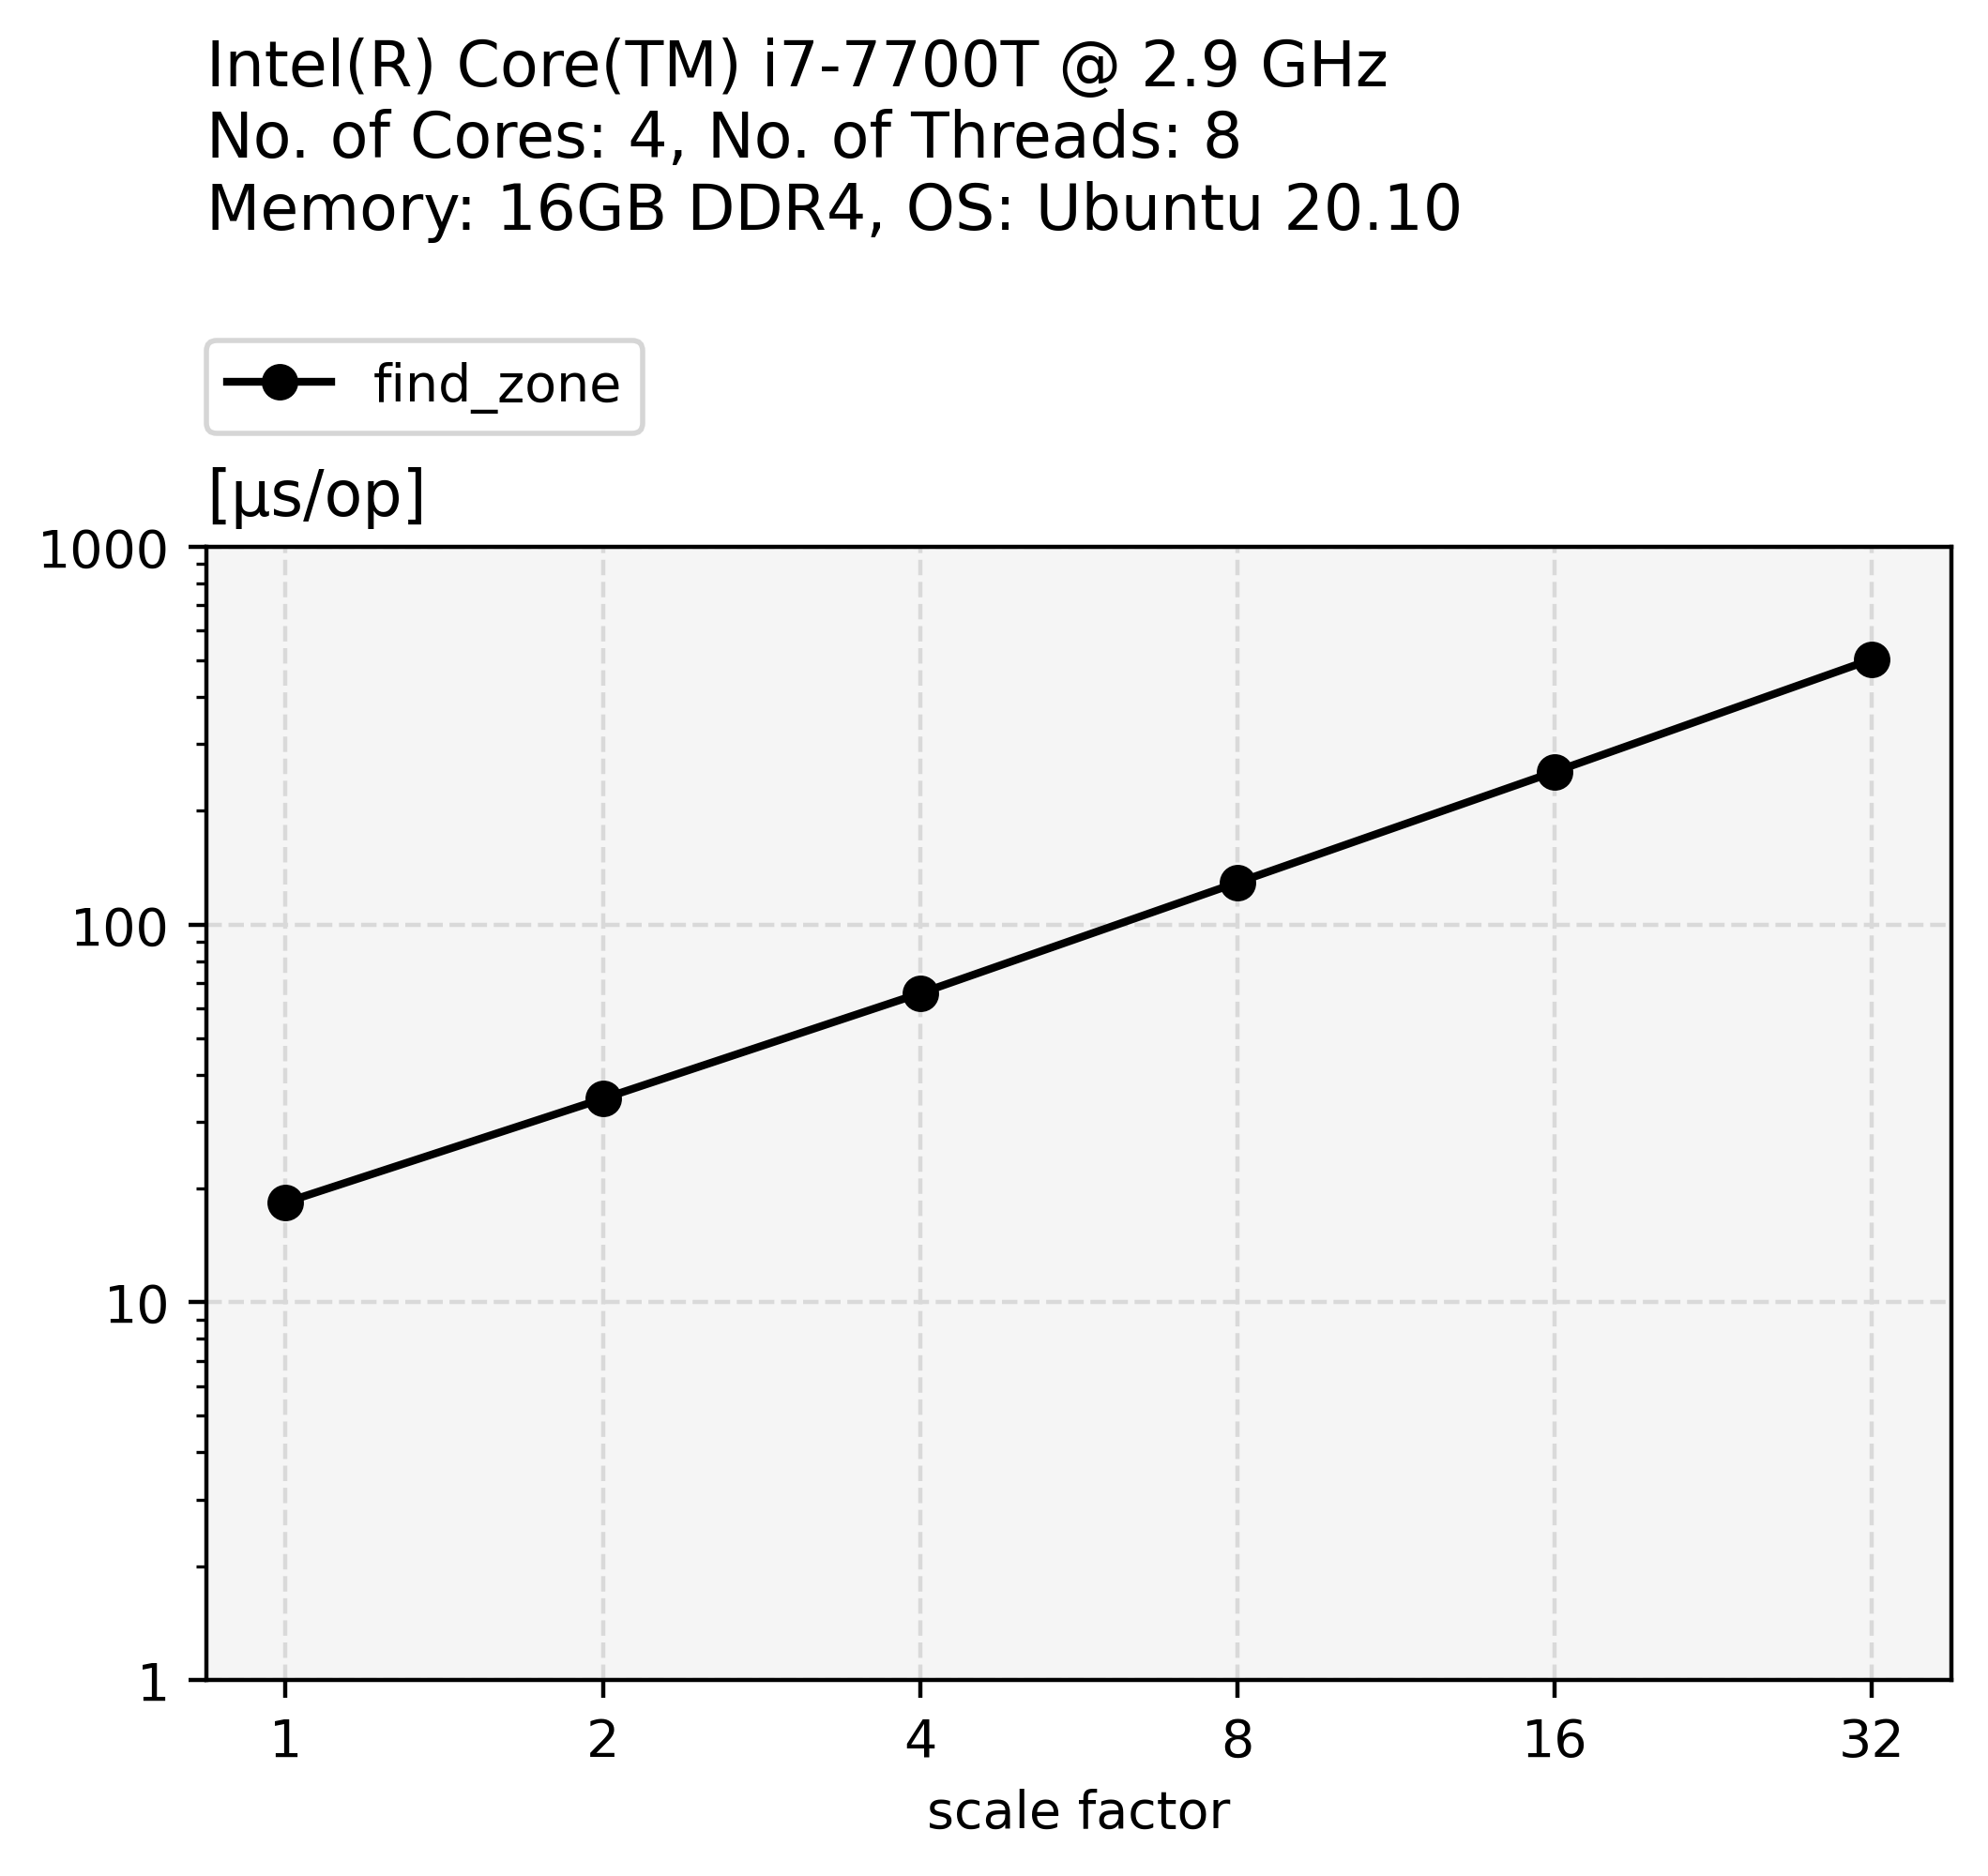
\includegraphics[width=\linewidth]{img/find_zone.png}
      \caption{\texttt{find\_zone} Function Scalability}
      \label{fig:sub: find zone Scalability}
    \end{subfigure}\hfill%
    \begin{subfigure}[t]{.22\textwidth}
      \centering
      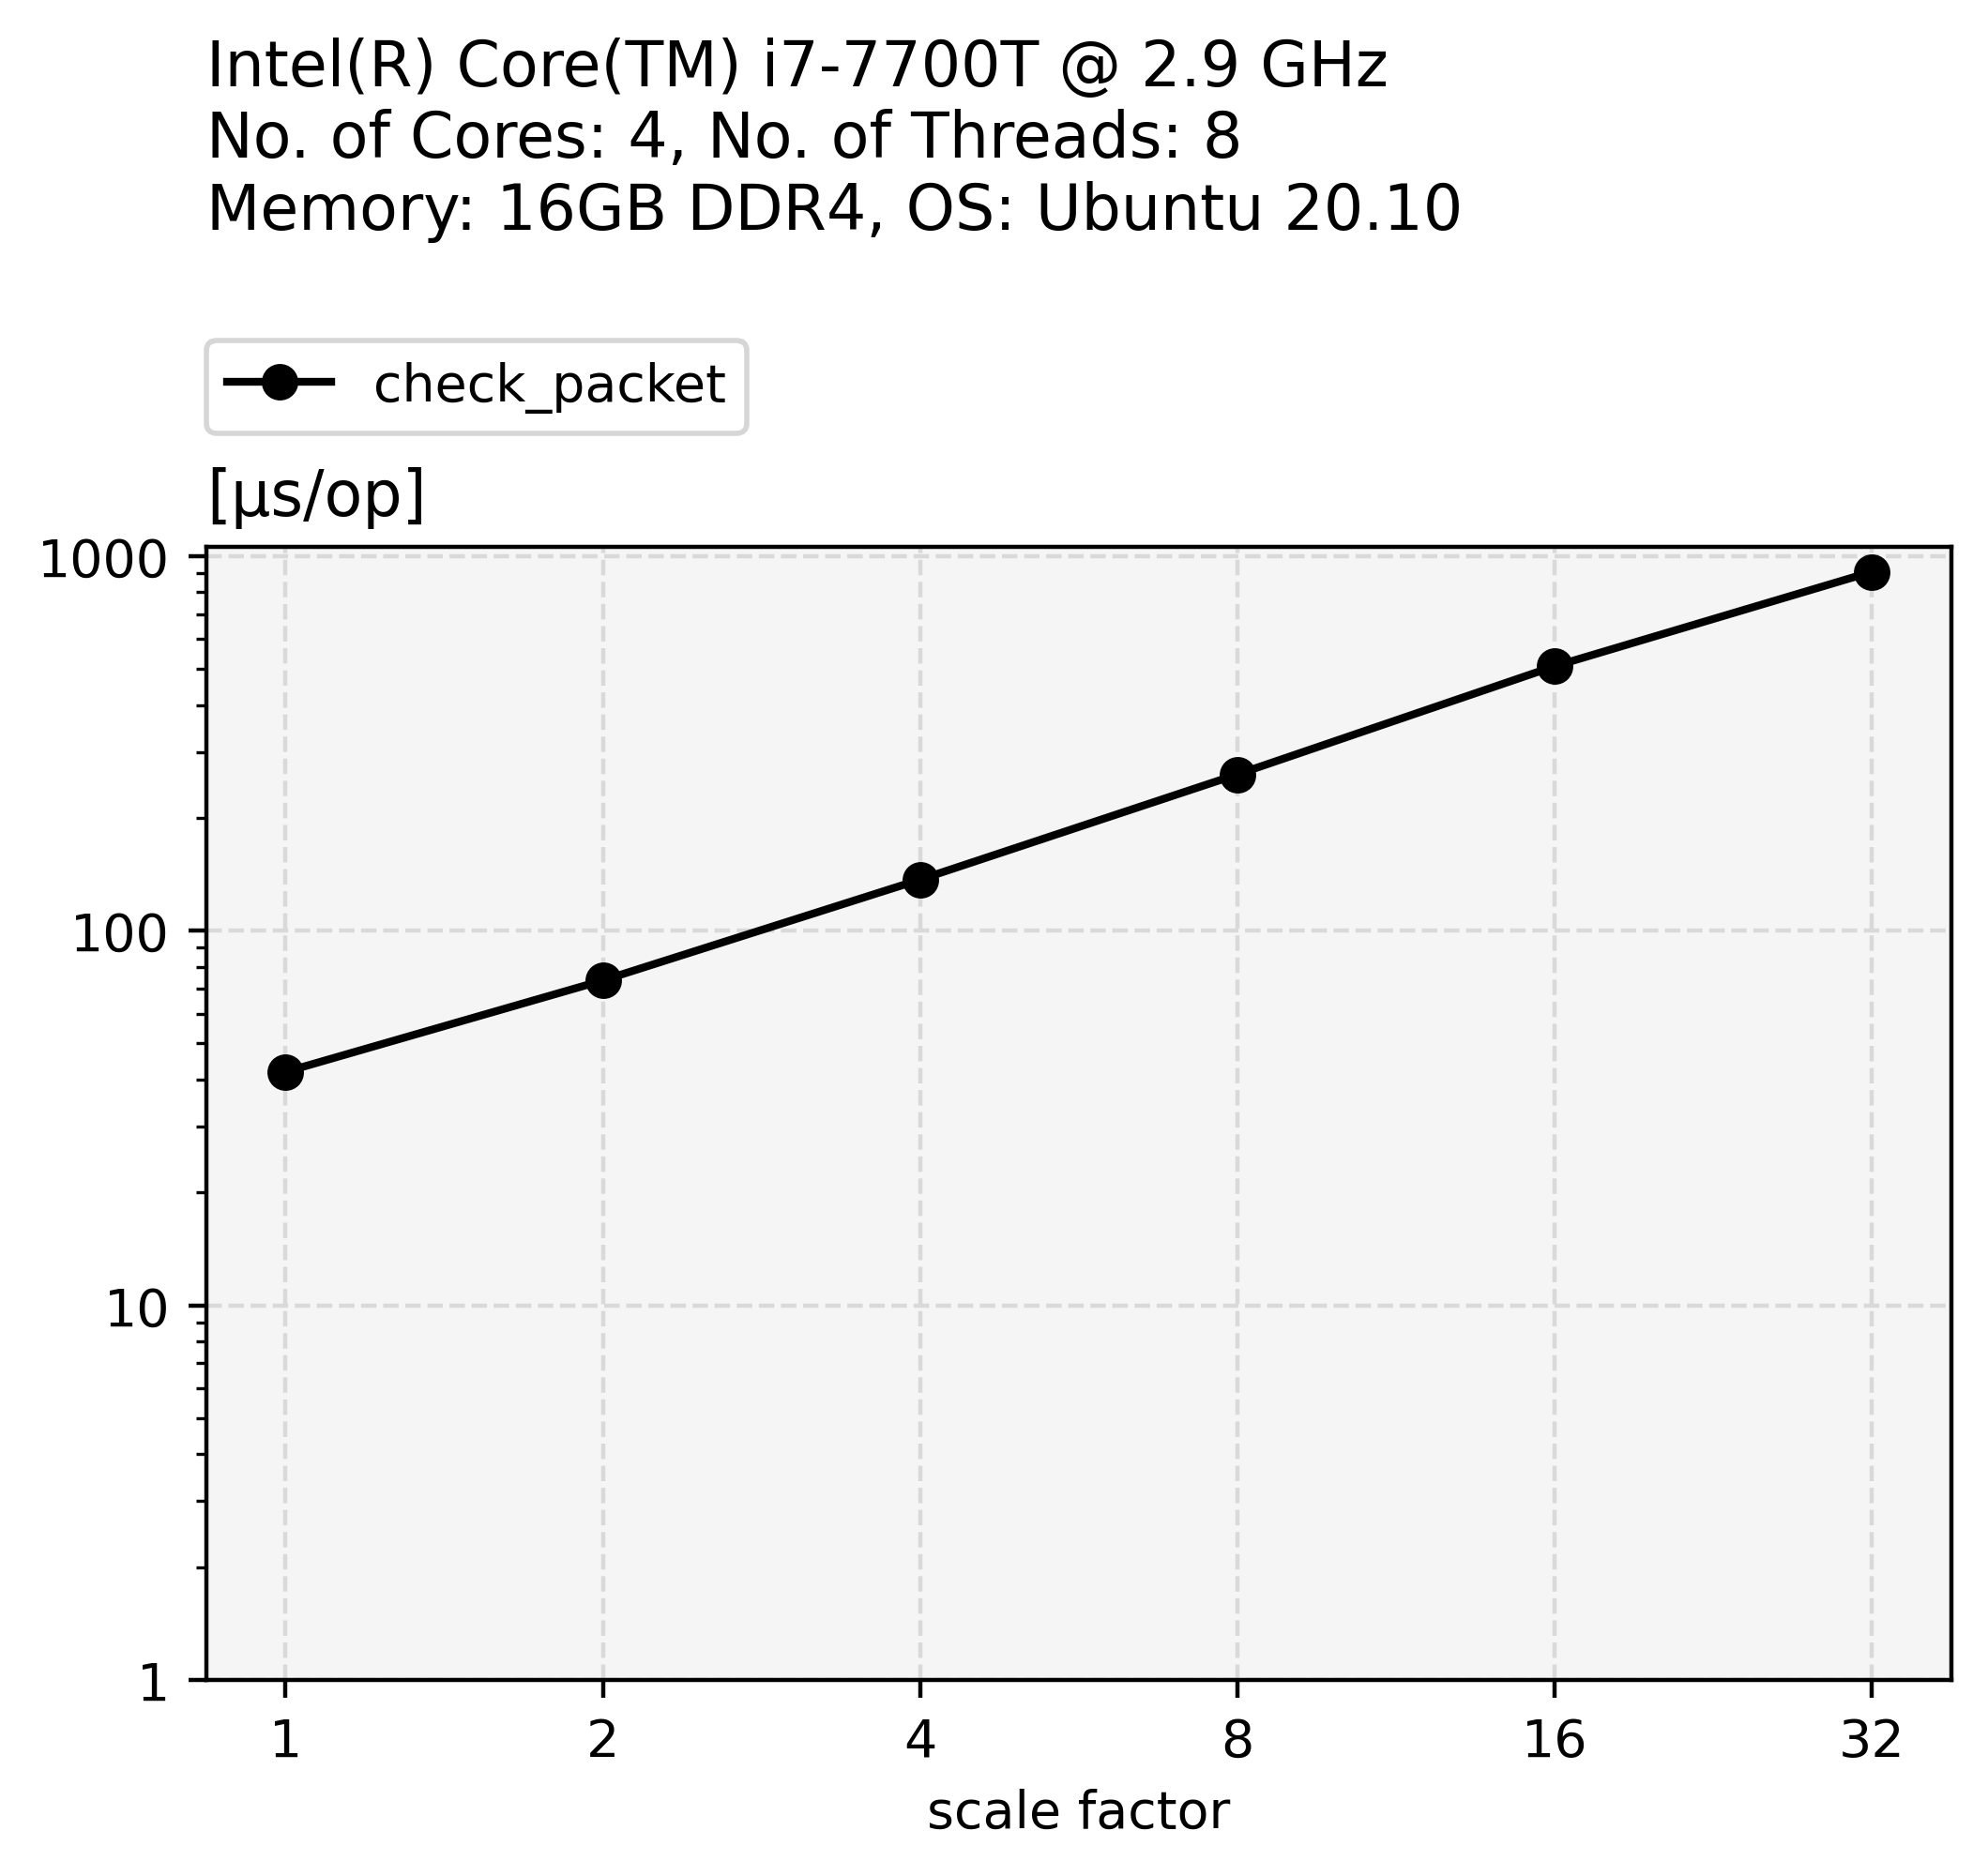
\includegraphics[width=\linewidth]{img/check_packet.png}
      \caption{\texttt{check\_packet} Function Scalability}
      \label{fig:sub: check packet Scalability}
    \end{subfigure}
    \caption{Endpoint \acs{TP} Scalability (Upscaling the number of subnets and policies)}
    \label{fig:Endpoint TP Scalability}
\end{figure}

\begin{figure}[t]
    \centering
    \begin{subfigure}[t]{.22\textwidth}
      \centering
      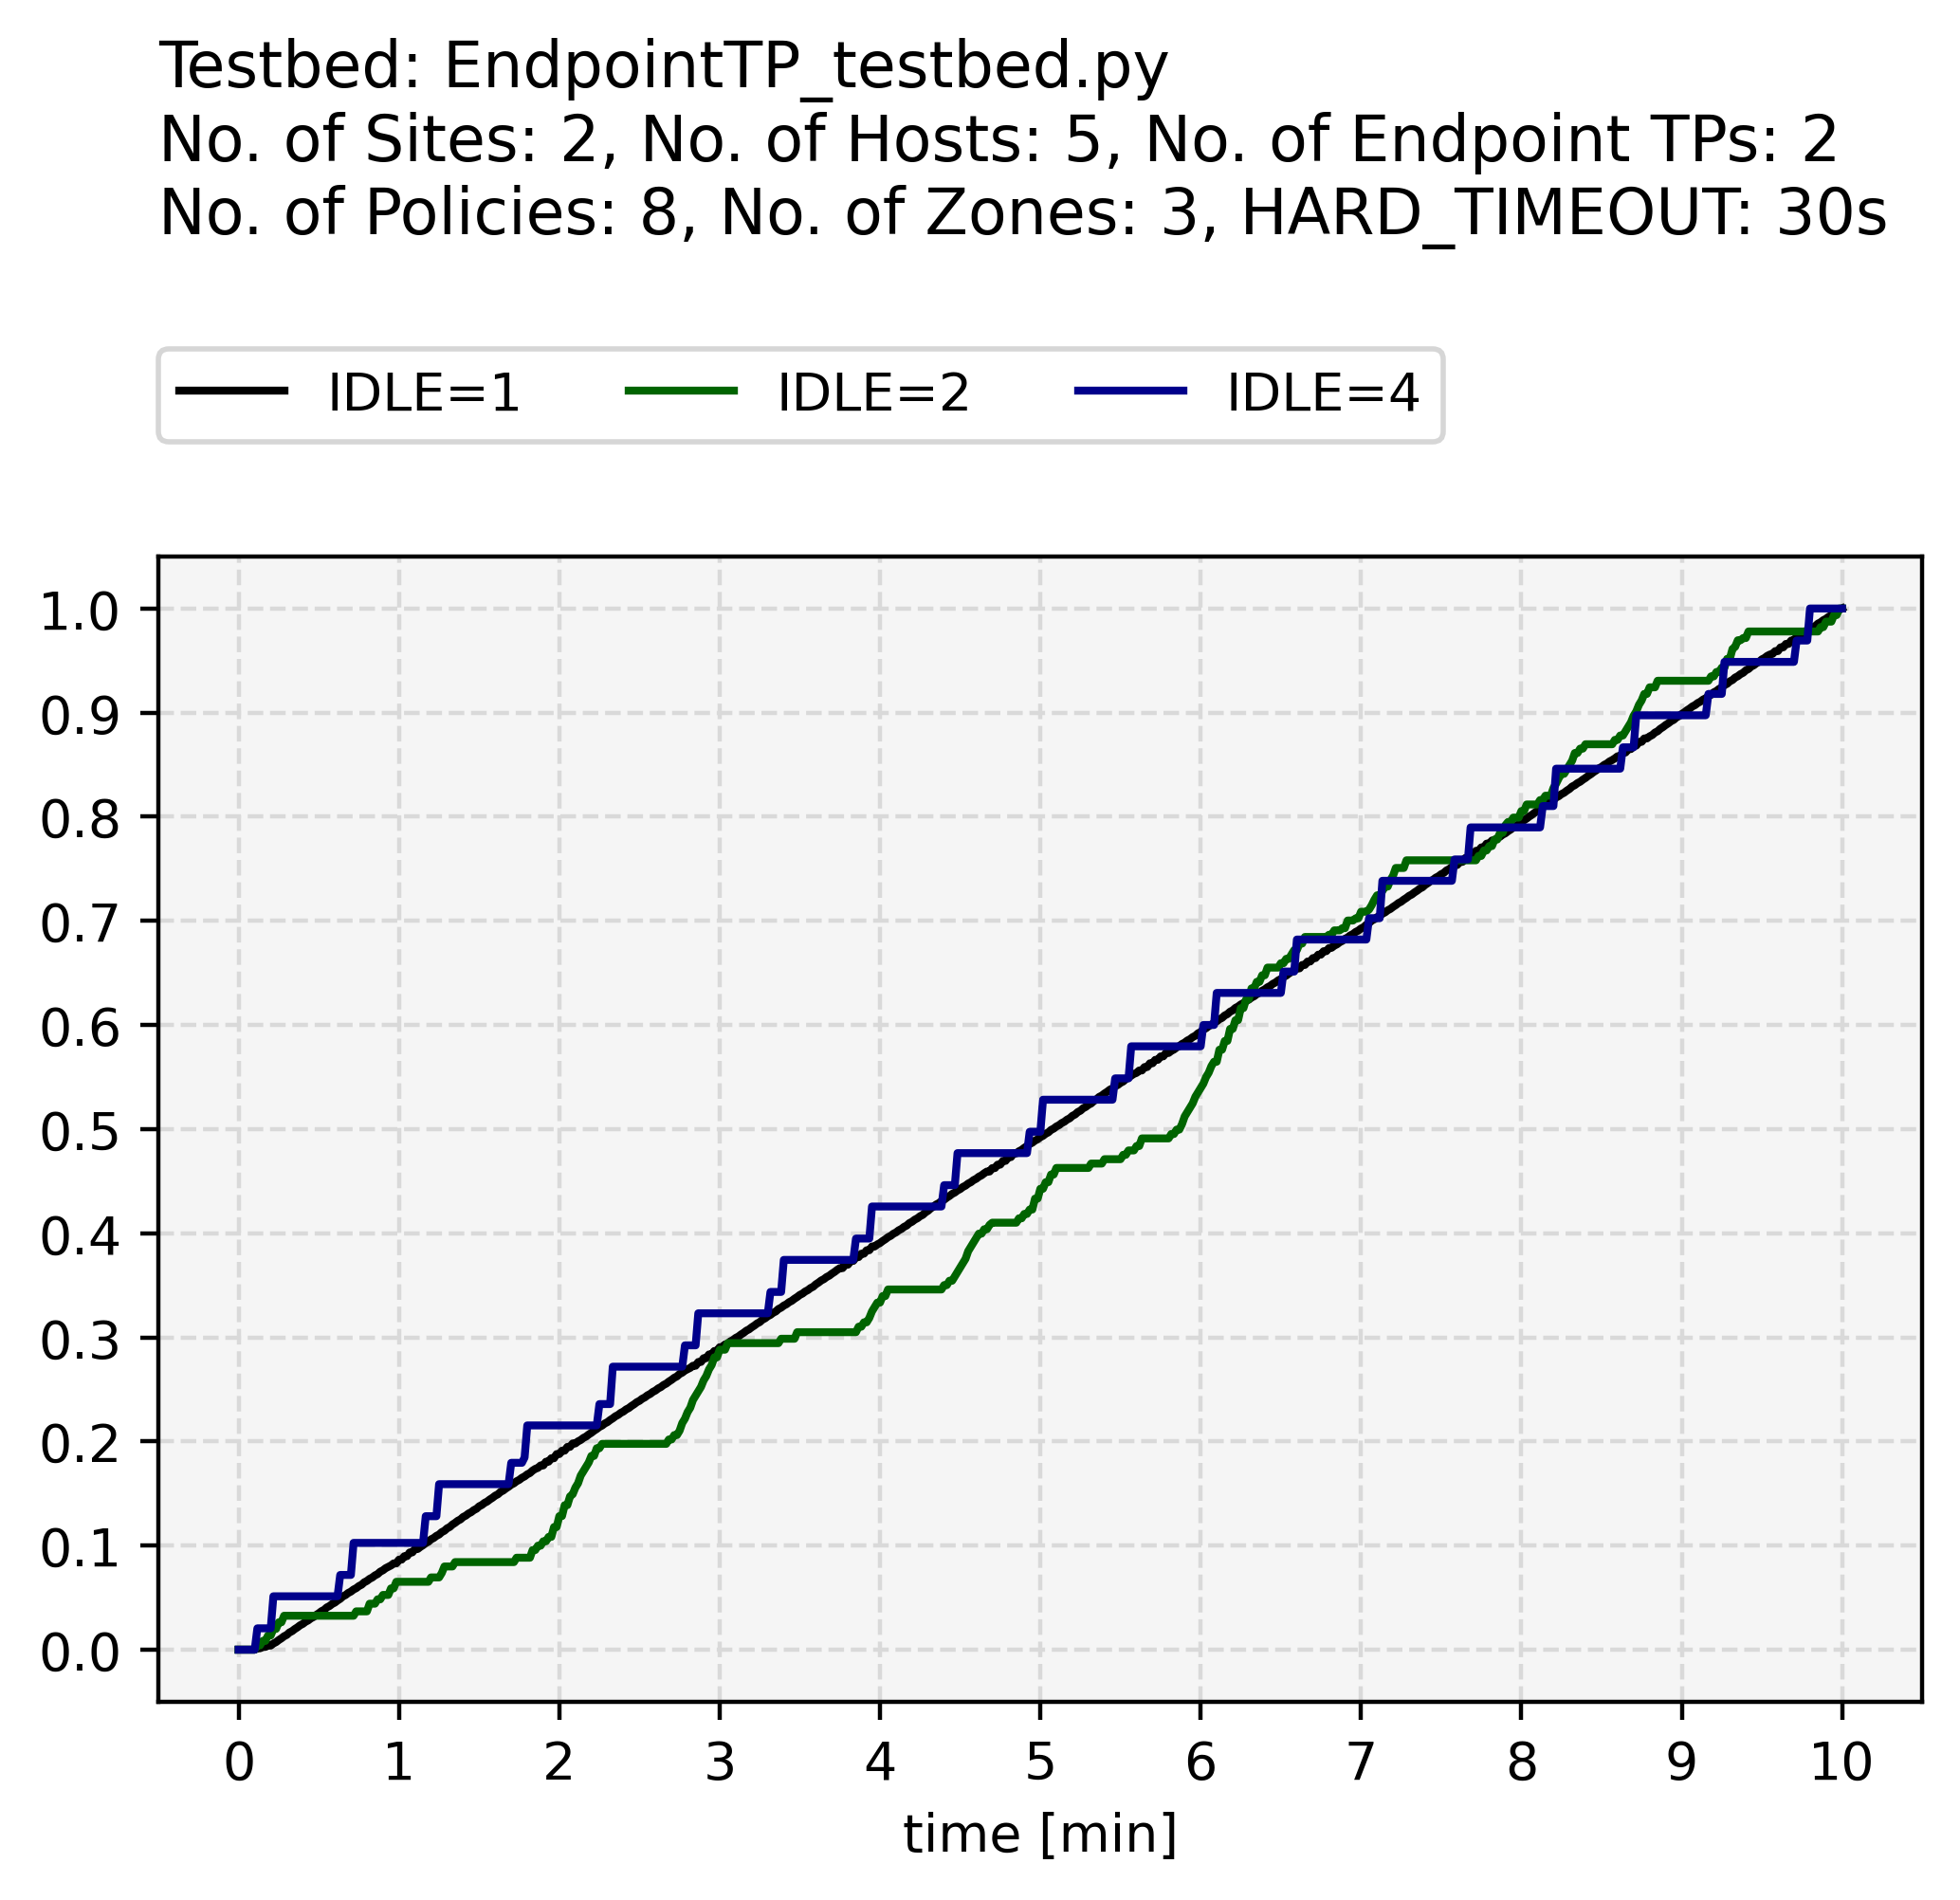
\includegraphics[width=\linewidth]{img/packet-in_idle_new_cdf.png}
      \caption{Varying \texttt{IDLE\_TIMEOUT}}
      \label{fig:sub: Varying IDLE_TIMEOUT}
    \end{subfigure}\hfill%
    \begin{subfigure}[t]{.22\textwidth}
      \centering
      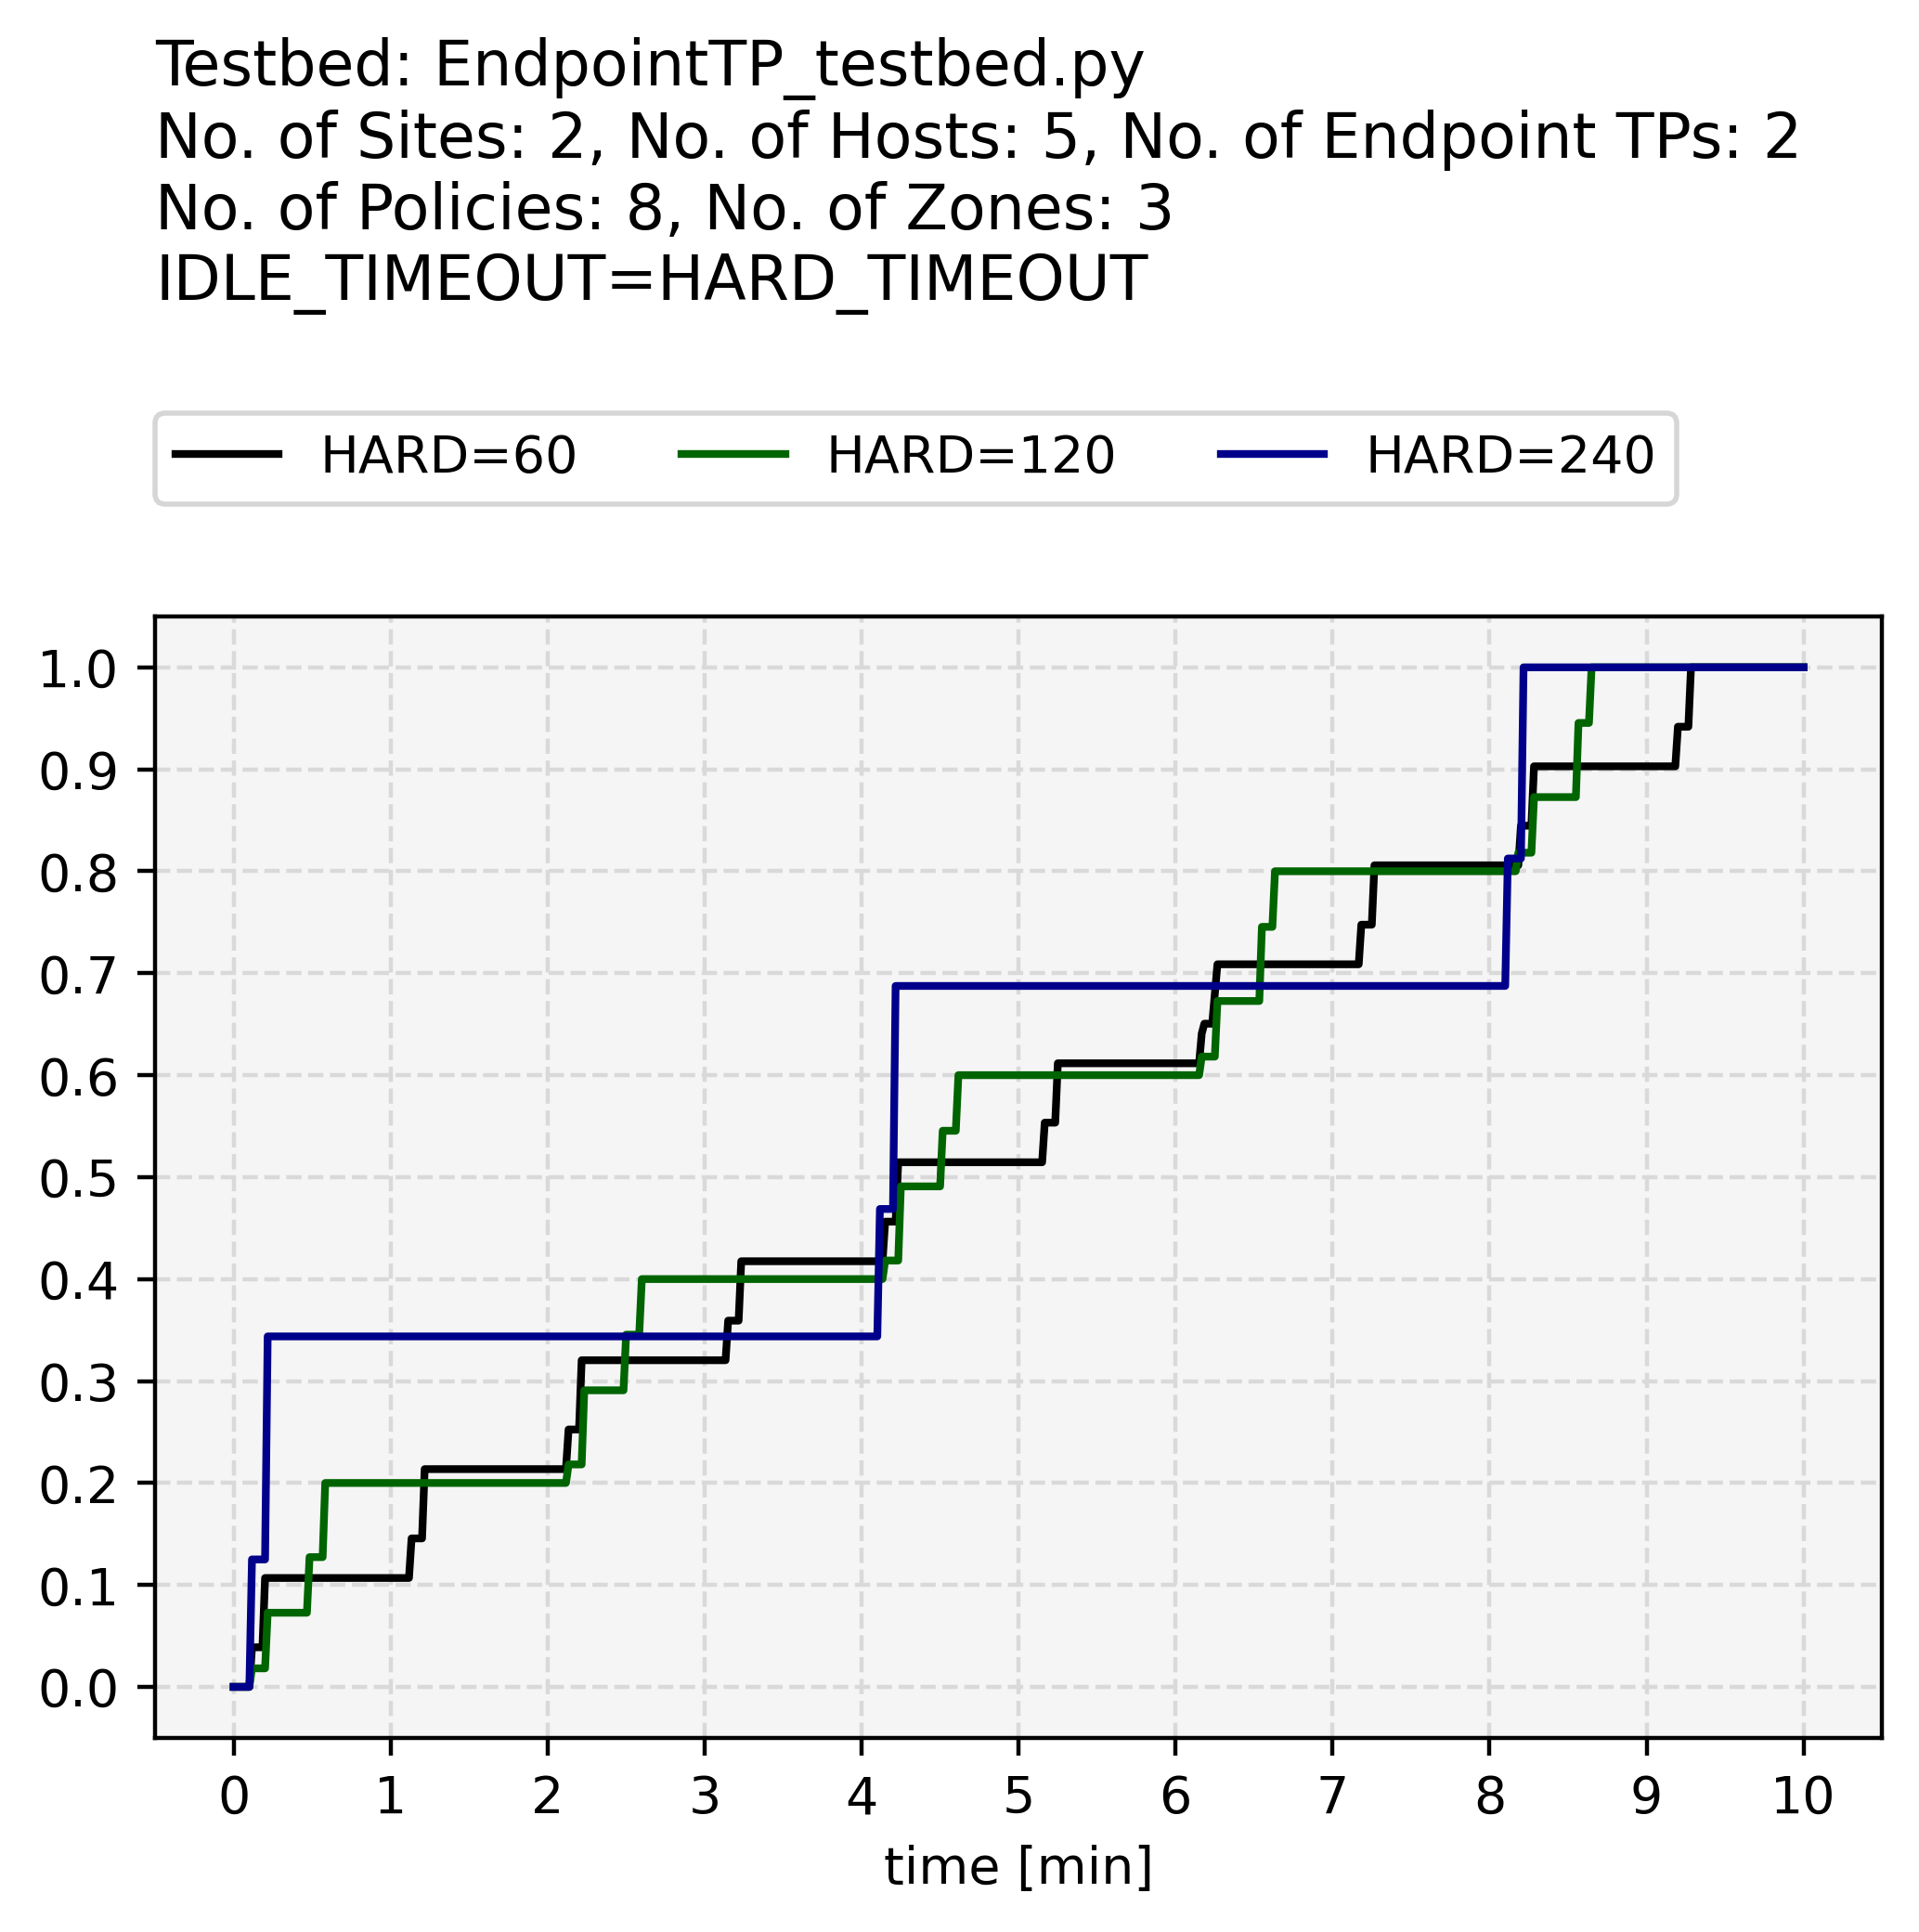
\includegraphics[width=\linewidth]{img/packet-in_hard_new_cdf.png}
      \caption{Varying \texttt{HARD\_TIMEOUT}}
      \label{fig:sub: Varying HARD_TIMEOUT}
    \end{subfigure}
    \caption{\acs{CDF} Plot of Packet-In Messages per Time (Sum of two instances of Endpoint \acsp{TP})}
    \label{fig:CDF Plot of Packet-In Messages per Time}
\end{figure}

Another factor that we should investigate when evaluating the performance of an Endpoint \acs{TP} is the workload it needs to be able to handle and what factors influence the magnitude of the workload. We measure the workload as the number of packet-in messages an Endpoint \acs{TP} needs to handle over time. Many factors, like the number of hosts, the type of traffic they generate, the complexity of the policy database or the presence of an attacker influence the workload. These factors are however hard to simulate and their effect can be controlled by scaling up or employing additional defense mechanisms, in case of an attacker being present. What however is of interest to us is how certain parameters we choose while deploying MONDRIAN affect the workload on the Endpoint \acs{TP}. For that we consider the two OpenFlow parameters \texttt{IDLE_TIMEOUT} and \texttt{HARD_TIMEOUT} and analyze how they should be chosen, depending on the desired properties a data center operator would like to achieve.

The \texttt{IDLE_TIMEOUT} should be chosen in a way, such that the flow table of an \acs{SDN} switch doesn't get exhausted. If a flow table is too full of flow table entries, then we should decrease the size of the \texttt{IDLE_TIMEOUT}. Otherwise, it's better to have an as big as possible \texttt{IDLE_TIMEOUT}, since we don't want to unnecessarily cause an \acs{SDN} switch to contact an Endpoint \acs{TP} only because a machine was inactive for some time. 

The \texttt{HARD_TIMEOUT} should also be chosen as big as possible, with the constraint that the \texttt{refresh_interval} of the Endpoint \acs{TP} added to the \texttt{HARD_TIMEOUT} doesn't exceed the responsiveness requirement to policy changes. The \texttt{HARD_TIMEOUT}'s responsibility is to make sure that flow table entries expire once they could be outdated.

In our experiment, we use the Endpoint \acs{TP} testbed with a traffic generator, which periodically lets all hosts of the same zone ping each other and then sleeps for two seconds to simulate idle time. With the \texttt{Stats} module we then measure the number of packet-in messages over a time period of 10 minutes.

In the \acs{CDF} (\acl{CDF}) plot in figure \ref{fig:sub: Varying IDLE_TIMEOUT} we show the results for \texttt{IDLE_TIMEOUT}s 1, 2 and 4 seconds. For \texttt{IDLE_TIMEOUT} = 1 we have a smooth line, meaning that we get a continuous stream of packet-in messages. This is because the timeout (1s) is smaller than the idle time (2s) we simulate. Hence, we get flow table misses in each round of the traffic generator. If the idle time (2s) is equal to the timeout (2s), we get a curvy line which isn't smooth nor spikey. This is because sometimes the idle time will be long enough to cause the flow table entries to be removed and sometimes it will be too short, depending on fluctuations in the performance of the testbed. If however the timeout (4s) is bigger than the idle time (2s), we get a sawtooth-shaped line with a step size of 30 seconds, which is the \texttt{HARD_TIMEOUT} in our experiment. This means that in this case the \texttt{IDLE_TIMEOUT} never had an effect, which is desirable for as long as the \acs{SDN} switches aren't exhausted. Like this we can determine the ideal \texttt{IDLE_TIMEOUT} for a specific kind of traffic. However, in our experiment we have artificially crafted traffic and real-world traffic can deviate arbitrarily from any artificially crafted traffic, making the choosing of ideal parameters a non-trivial problem. 

Figure \ref{fig:sub: Varying HARD_TIMEOUT} shows a \acs{CDF} plot where we vary the values for the \texttt{HARD_TIMEOUT} from 1 minute to 2 and 4 minutes. As we expect, all lines are sawtooth-shaped with the corresponding timeout length as a step size. Bigger steps, meaning bigger \texttt{HARD_TIMEOUT}s, mean that less packet-in messages will be received and are therefore desirable. However, as previously mentioned with increasing \texttt{HARD_TIMEOUT}s, we lower the responsiveness of the MONDRIAN deployment, which at some point might be inacceptable.

Conclusively, one can say that the \texttt{HARD_TIMEOUT} should be chosen as large as acceptable with regards to the responsiveness of the system, whereas the \texttt{IDLE_TIMEOUT} should be chosen as large as possible for as long as no \acs{SDN} switches are exhausted. Overall, with reasonably chosen parameters, the Endpoint \acs{TP} will for sure be performant enough to not be the performance bottleneck on the data path.

%\todo{\\
%    - Performance good due to Openflow switches \\
%    - Get measurements and discuss them here (packet-in msg per workload depending on some parameters)\\
%    - Result: Performance is good meaning it won't be the bottleneck
%}

\FloatBarrier
\subsubsection{Gateway TP}
The Gateway \acs{TP} is much more performance critical, since it has to process every single packet, which is intended for a host in a different domain. We are mainly interested in the throughput and the latency of the Gateway \acs{TP} and in locating the performance bottlenecks.

Figure \ref{fig:Performance of MONDRIAN Conversion Functions} shows both the time a conversion to and from a MONDRIAN packet takes, as well as the throughput of these conversion functions. We can see that the \texttt{FromMondrian} operation is about 1.2x faster than the \texttt{ToMondrian} operation and has an approximately 2.5x higher throughput than its counterpart. The reason, why the \texttt{FromMondrian} operation is considerably more performant, is that the MONDRIAN packet carries all information used for the transformation already in the header, while the gathering of this information in the \texttt{ToMondrian} operation is costly, especially since it involves parsing and serializing more data. In general, these memory intensive gopacket operations are the major performance bottleneck as we can see if we optimize the conversion operations, such that we can avoid some of these operations.

As shown in figure \ref{fig:Performance Improvement in ToMondrianAndSend} and \ref{fig:Performance Improvement in FromMondrianAndSend}, we can achieve a speedup of 1.72x and 1.85x in the functions \texttt{ToMondrianAndSend} and \texttt{FromMondrianAndSend} respectively, by avoiding to serialize a buffer into a gopacket, just to then read out the buffer of the packet in order to send it in the sending process.

The fact that such a simple gopacket related optimization causes a significant speedup, is a strong indicator that the gopackets are a major performance bottleneck. By analyzing the code with the Go profiler called \texttt{pprof}, we can see that apart from the gopacket related inefficiencies the next severe performance bottlenecks are the cryptographic operations. This was to be expected and is also good news since both of the aforementioned inefficiencies will naturally be avoided in production level code, since there we would be using more performant frameworks such as \acs{DPDK}, which minimizes the number of copying operations and has support for hardware accelerated cryptographic operations.

Conclusively, we can say that the benchmarking results are acceptable for a \acs{PoC} implementation, where fast prototyping was more important than the ability to write production level code. Furthermore, the design of the Gateway \acs{TP} is very minimalistic, which means that a production level implementation is expected to be able to compete performance wise with other commercial products in the same field such as \acs{VPN} solutions. 

%\todo{\\
%    - Microbenchmarking different functions \\
%    - Two performance penalties 1. gopackets 2. crypto -- both can be resolved in production level code with for example using DPDK \\
%    - Result: POC implementation shows limited performance due to gopackets/pcap but 
%    it can be implemented using DPDK and compete with commercial alternatives 
%    (Not done because too complicated for POC implementation -- fast prototyping was more important)
%}

\begin{figure}[t]
    \centering
    \begin{subfigure}[t]{.22\textwidth}
      \centering
      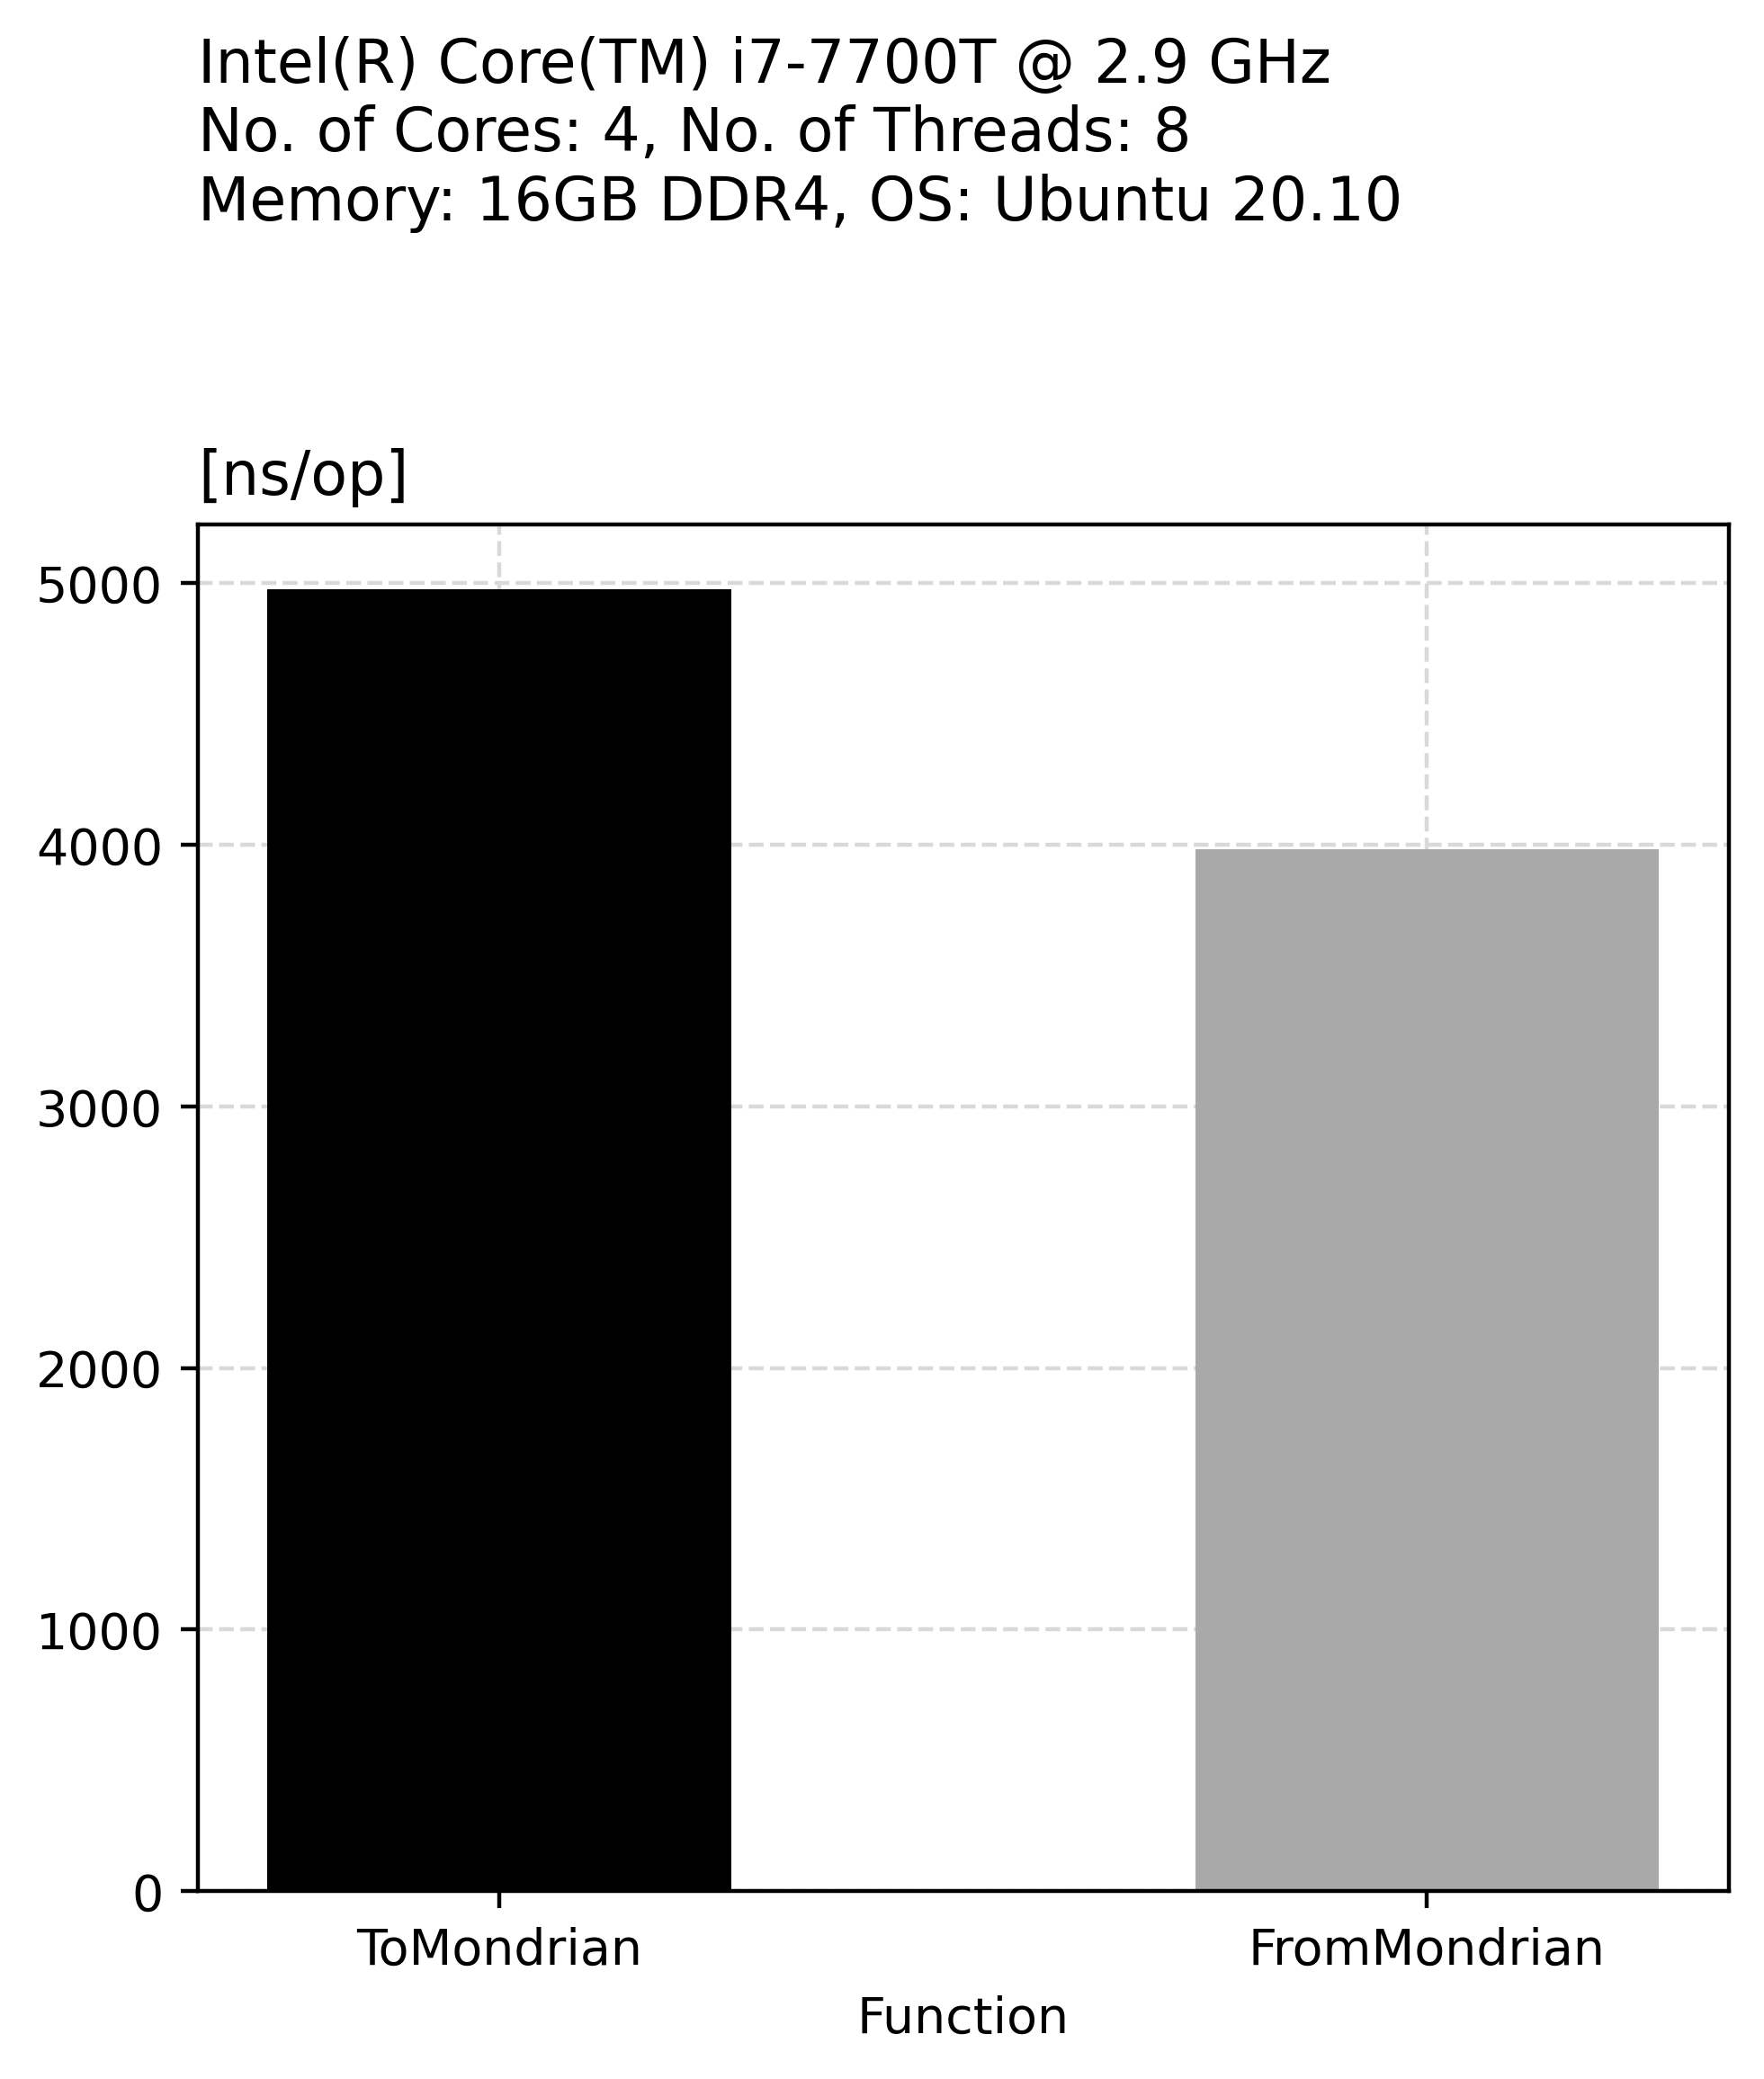
\includegraphics[width=\linewidth]{img/mondrian_transform_time.png}
      \caption{Time per Operation}
      \label{fig:sub: Time per Operation}
    \end{subfigure}\hfill%
    \begin{subfigure}[t]{.22\textwidth}
      \centering
      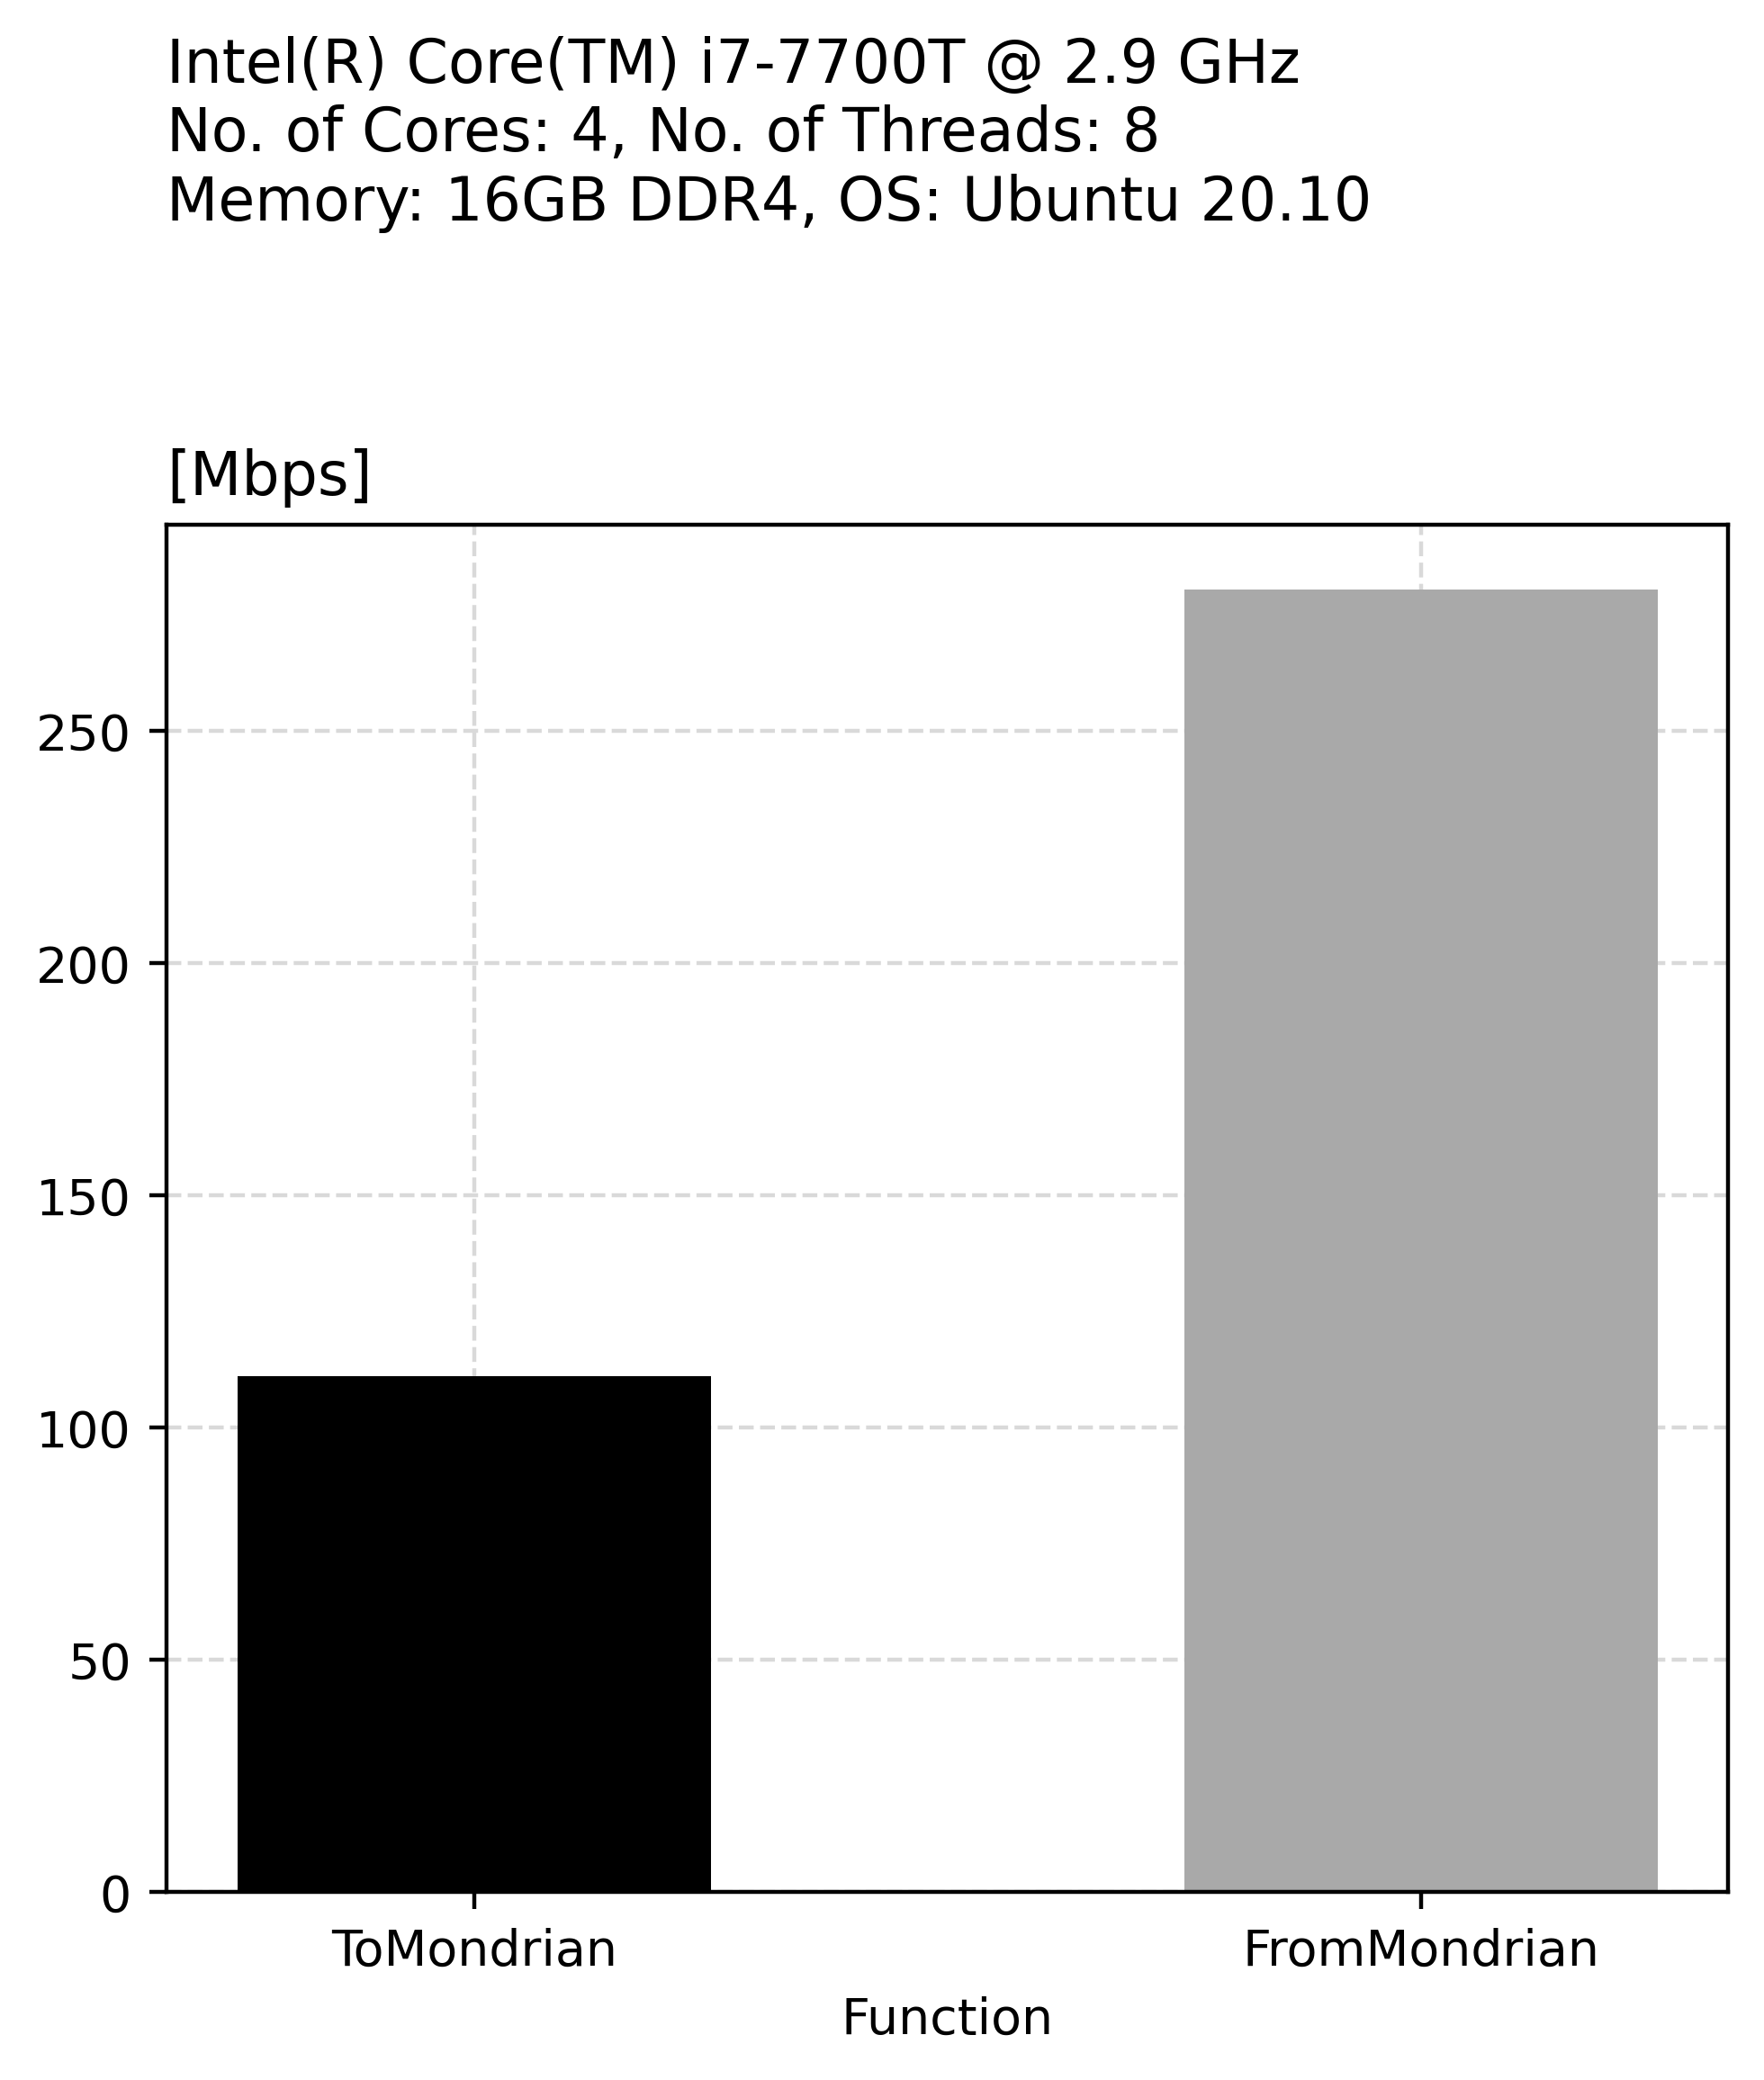
\includegraphics[width=\linewidth]{img/mondrian_transform_throughput.png}
      \caption{Throughput per Operation}
      \label{fig:sub: Throughput per Operation}
    \end{subfigure}
    \caption{Microbenchmarking Results of the MONDRIAN Conversion Functions}
    \label{fig:Performance of MONDRIAN Conversion Functions}
\end{figure}

\begin{figure}[t]
    \centering
    \begin{subfigure}[t]{.22\textwidth}
      \centering
      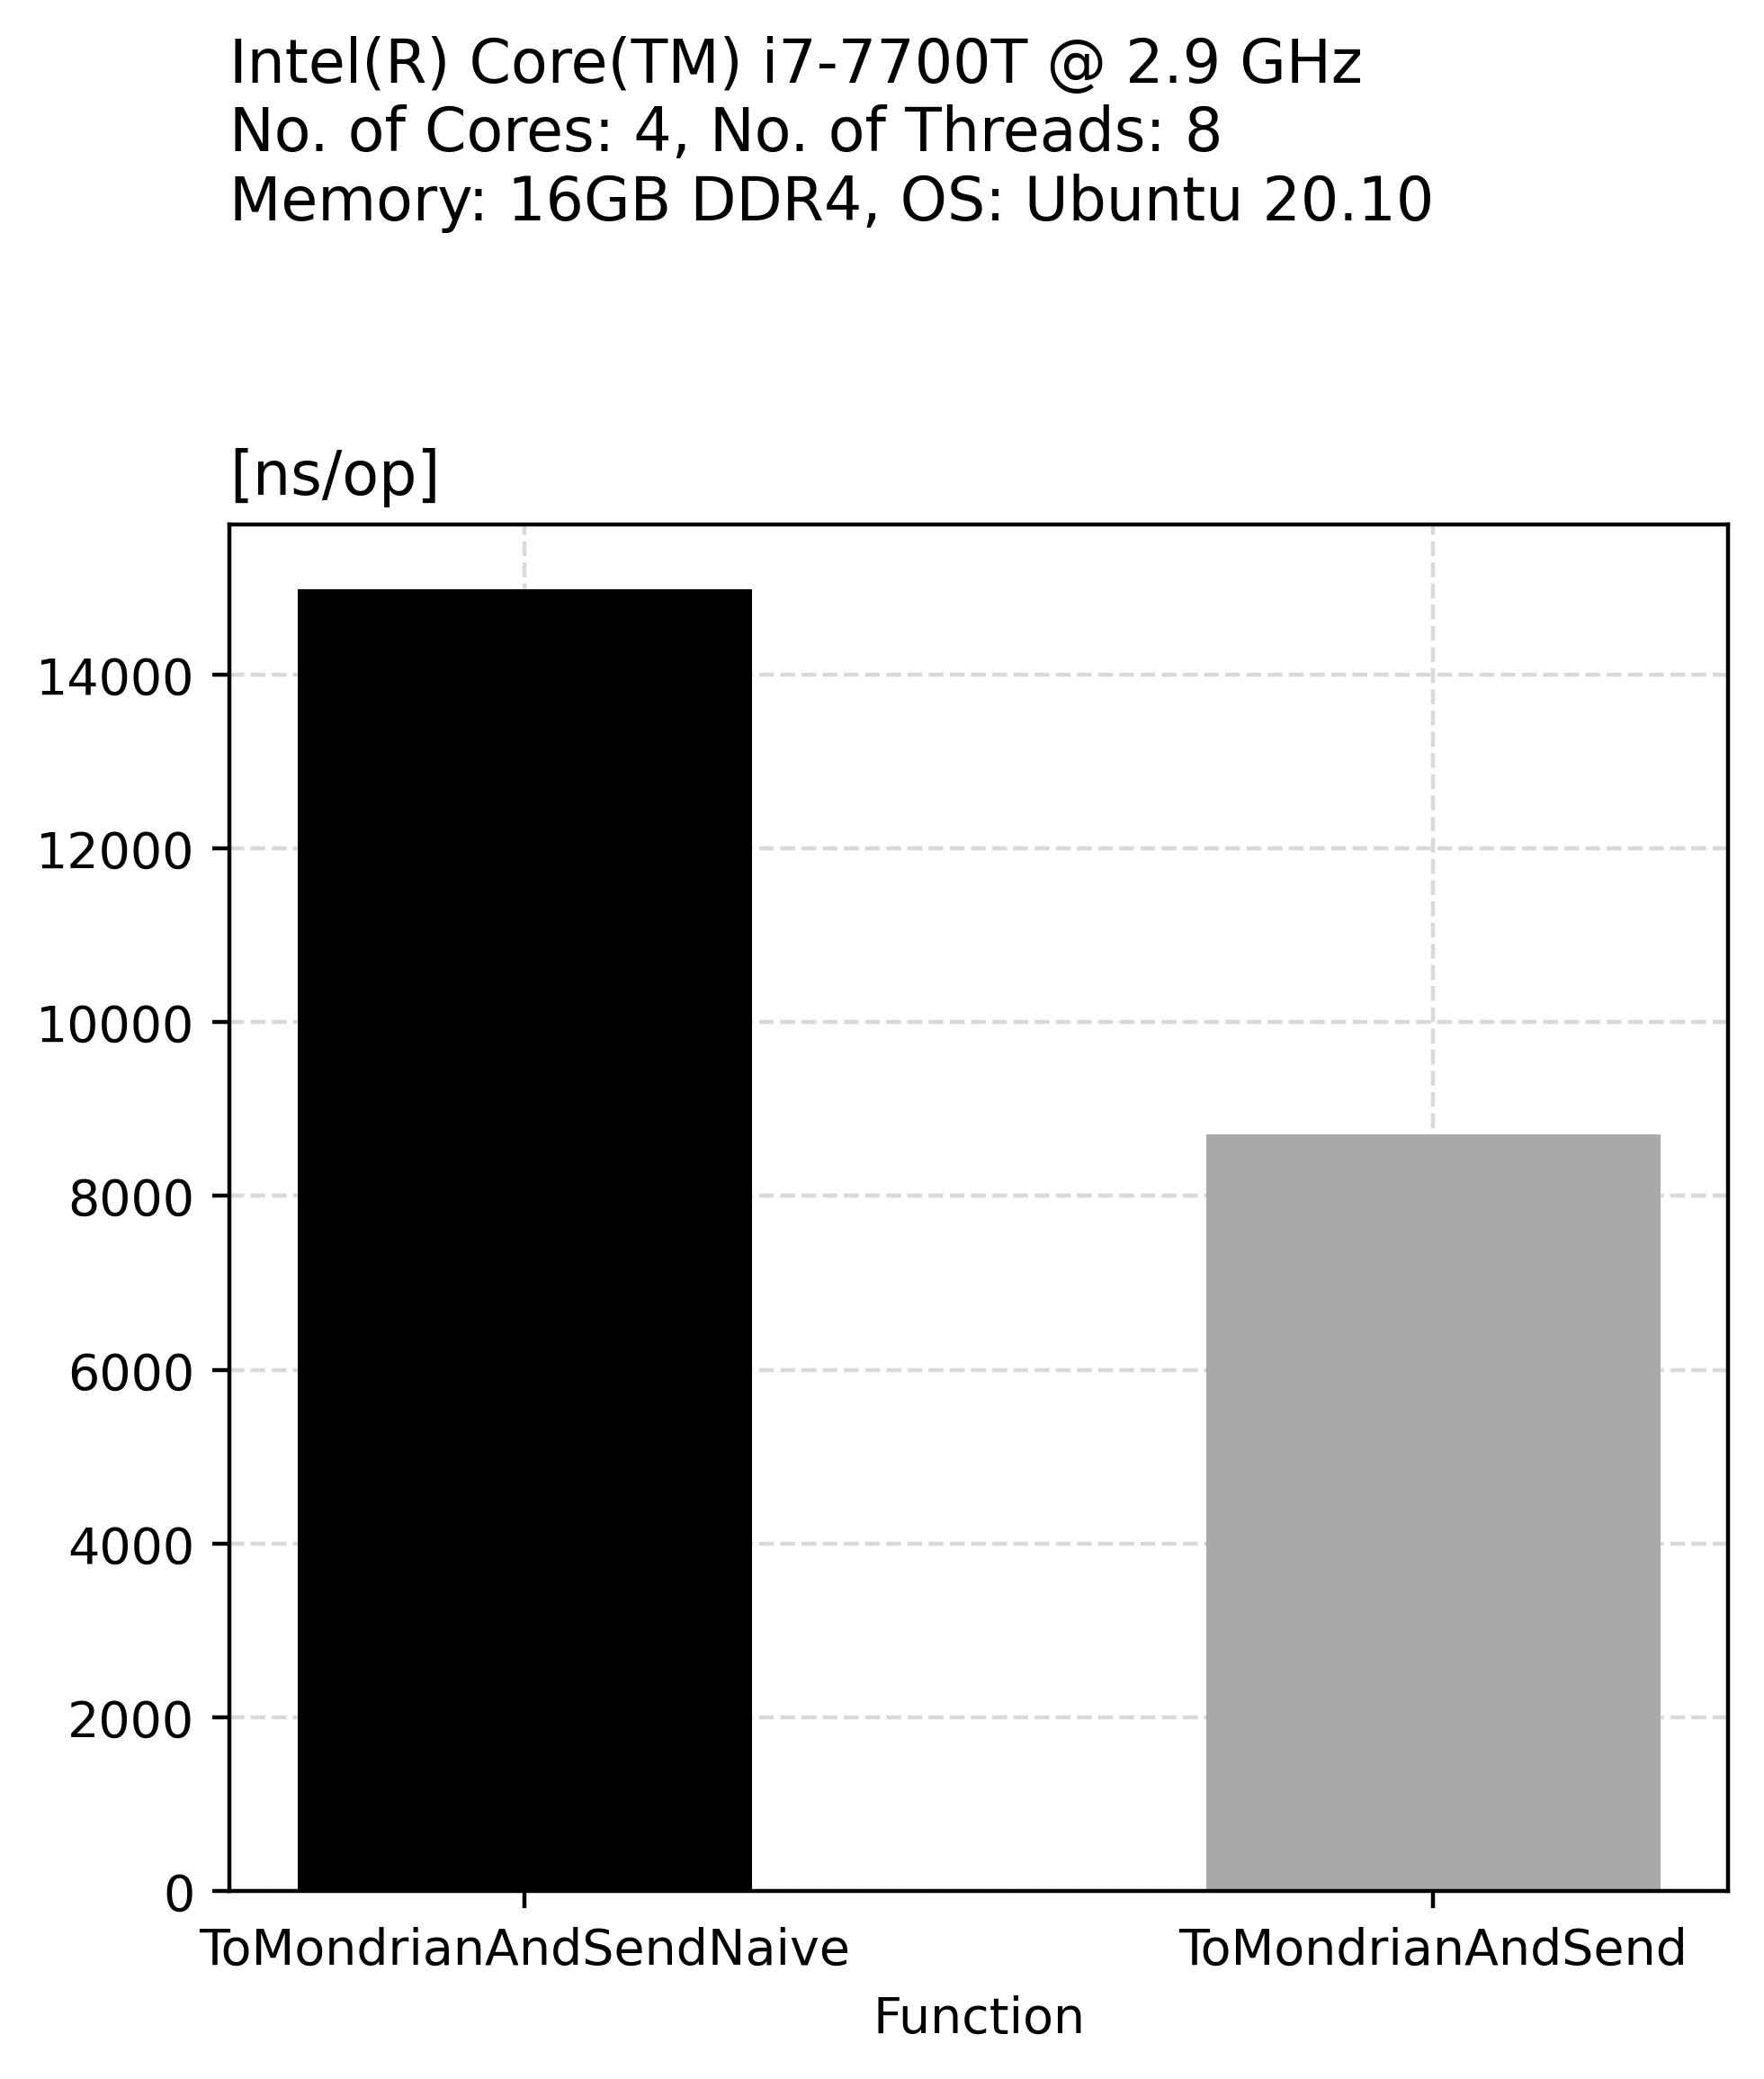
\includegraphics[width=\linewidth]{img/to_mondrian_and_send_opt_time.png}
      \caption{Latency Improvement}
      \label{fig:sub: Latency Improvement}
    \end{subfigure}\hfill%
    \begin{subfigure}[t]{.22\textwidth}
      \centering
      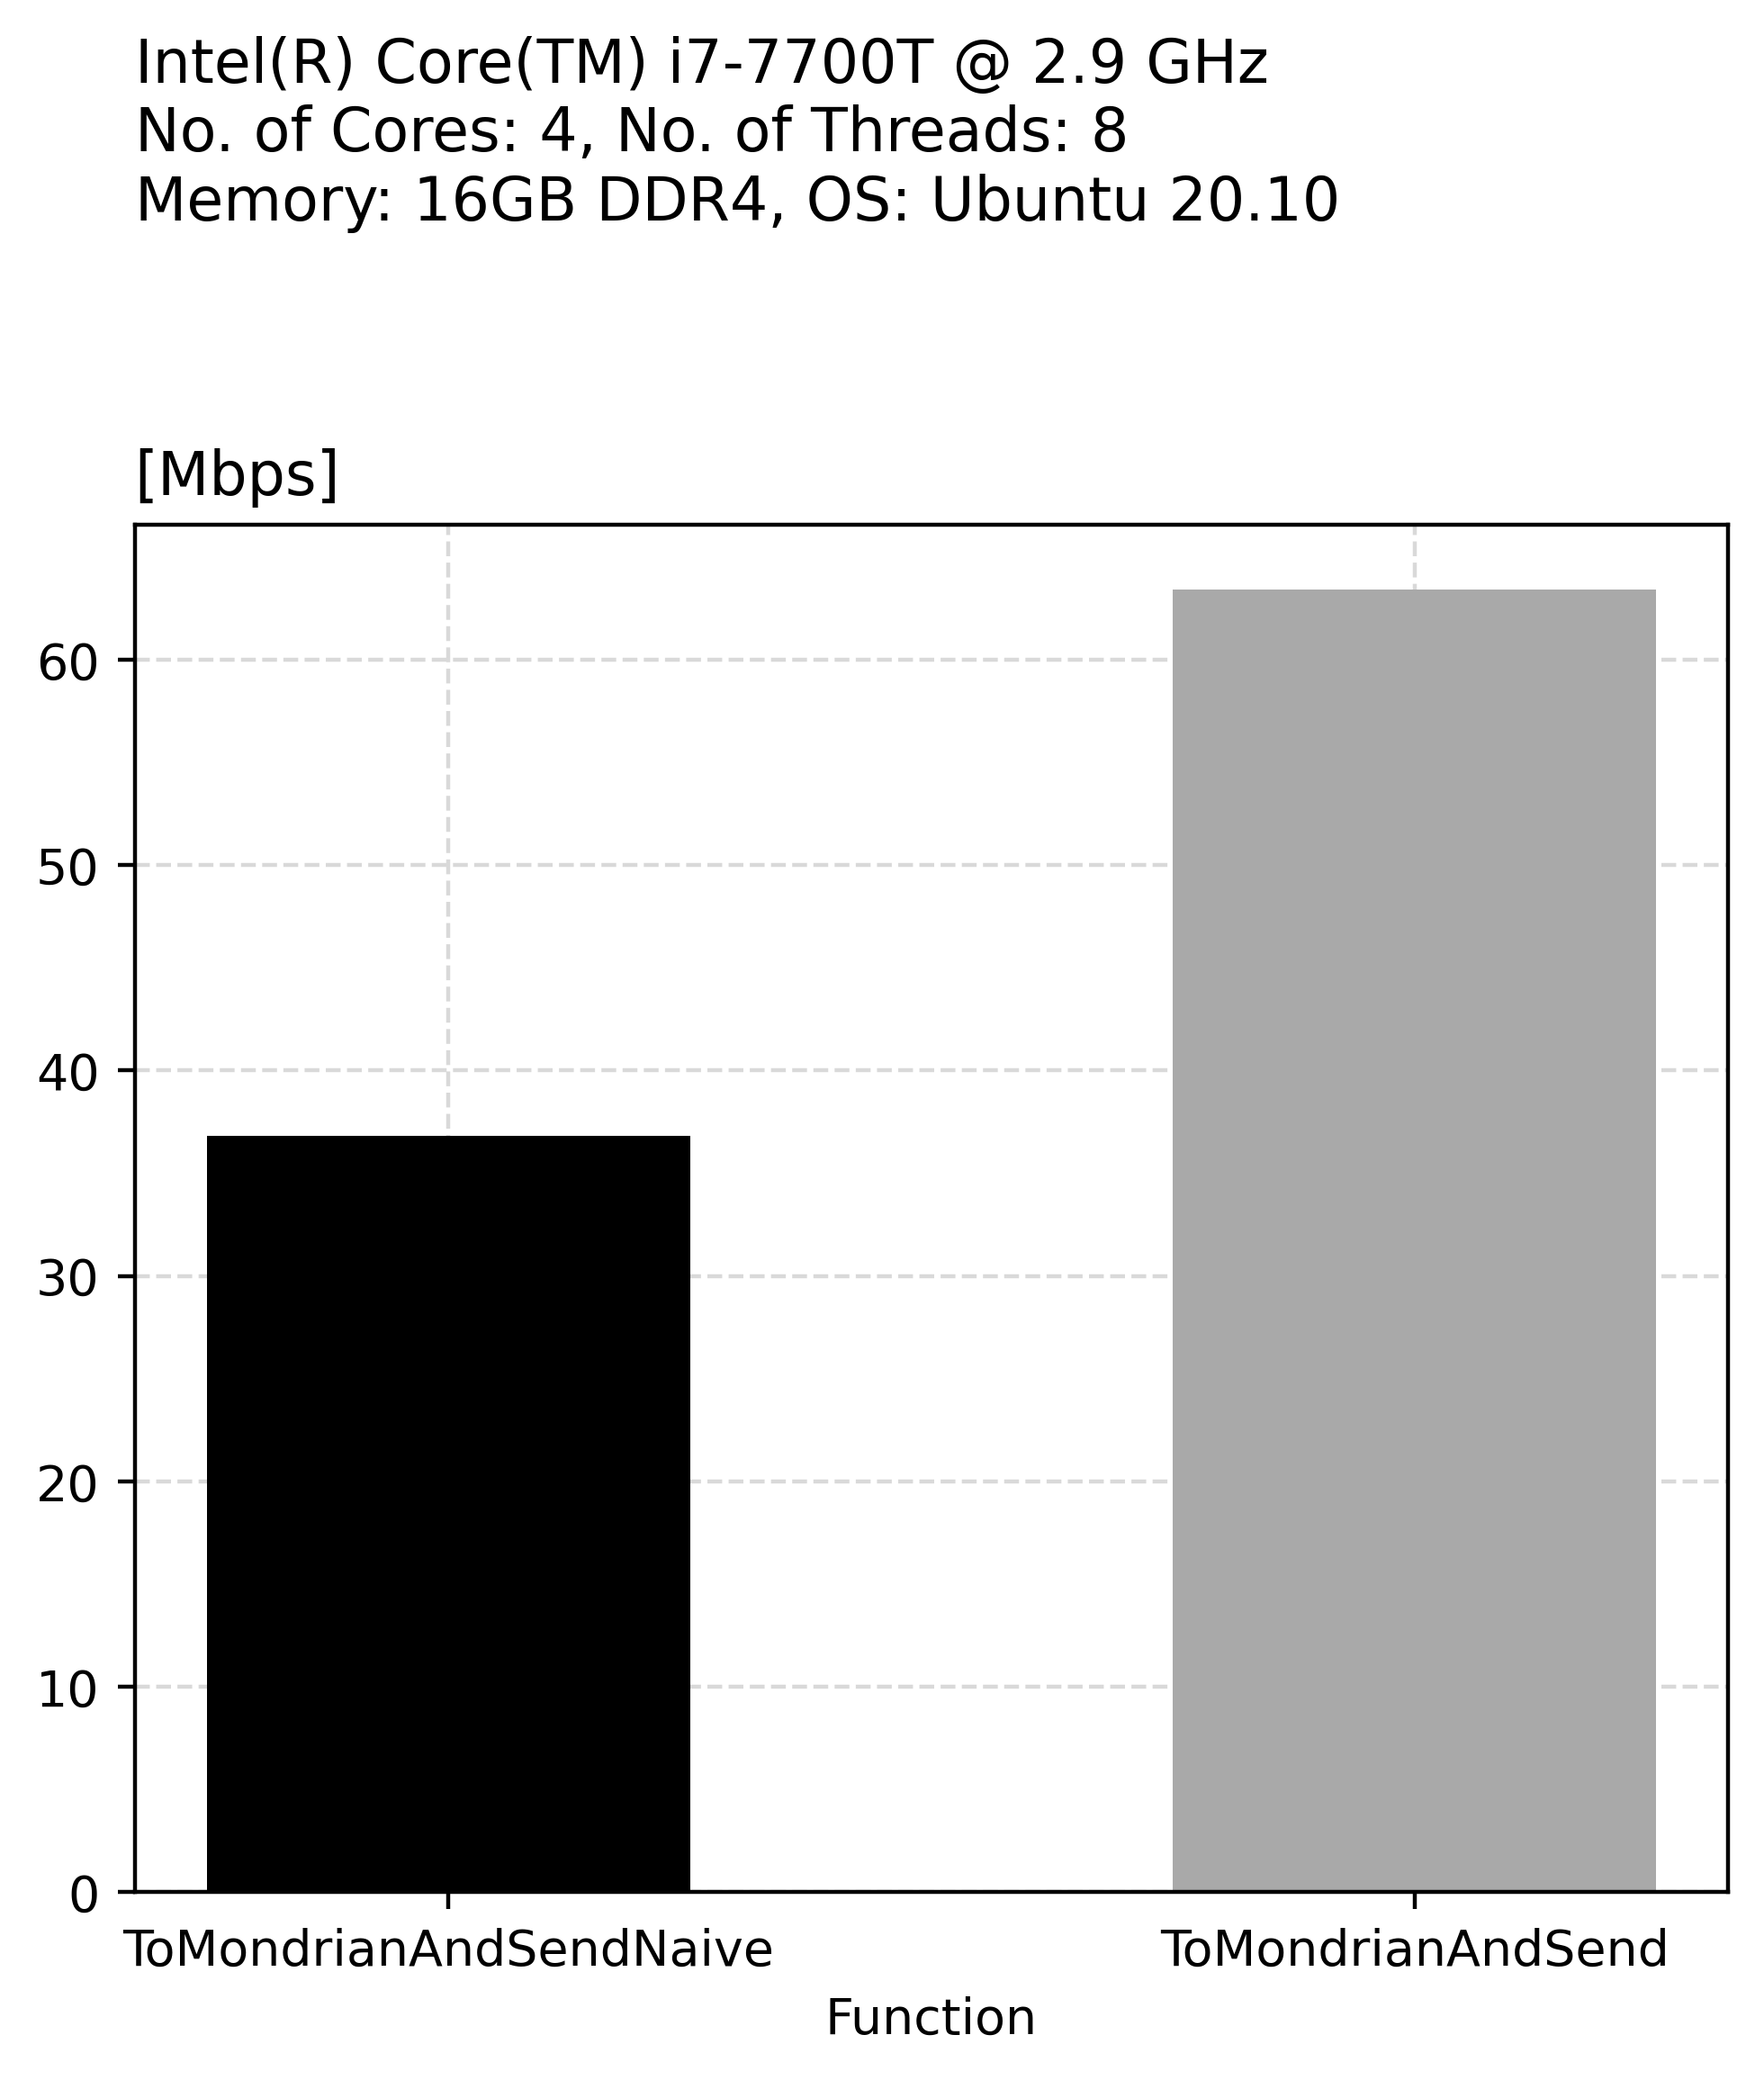
\includegraphics[width=\linewidth]{img/to_mondrian_and_send_opt_throughput.png}
      \caption{Throughput Improvement}
      \label{fig:sub: Throughput Improvement}
    \end{subfigure}
    \caption{Microbenchmarking Results of the Performance Improvement in \texttt{ToMondrianAndSend} (thanks to \texttt{gopacket} related optimizations)}
    \label{fig:Performance Improvement in ToMondrianAndSend}
\end{figure}

\begin{figure}[t]
    \centering
    \begin{subfigure}[t]{.22\textwidth}
      \centering
      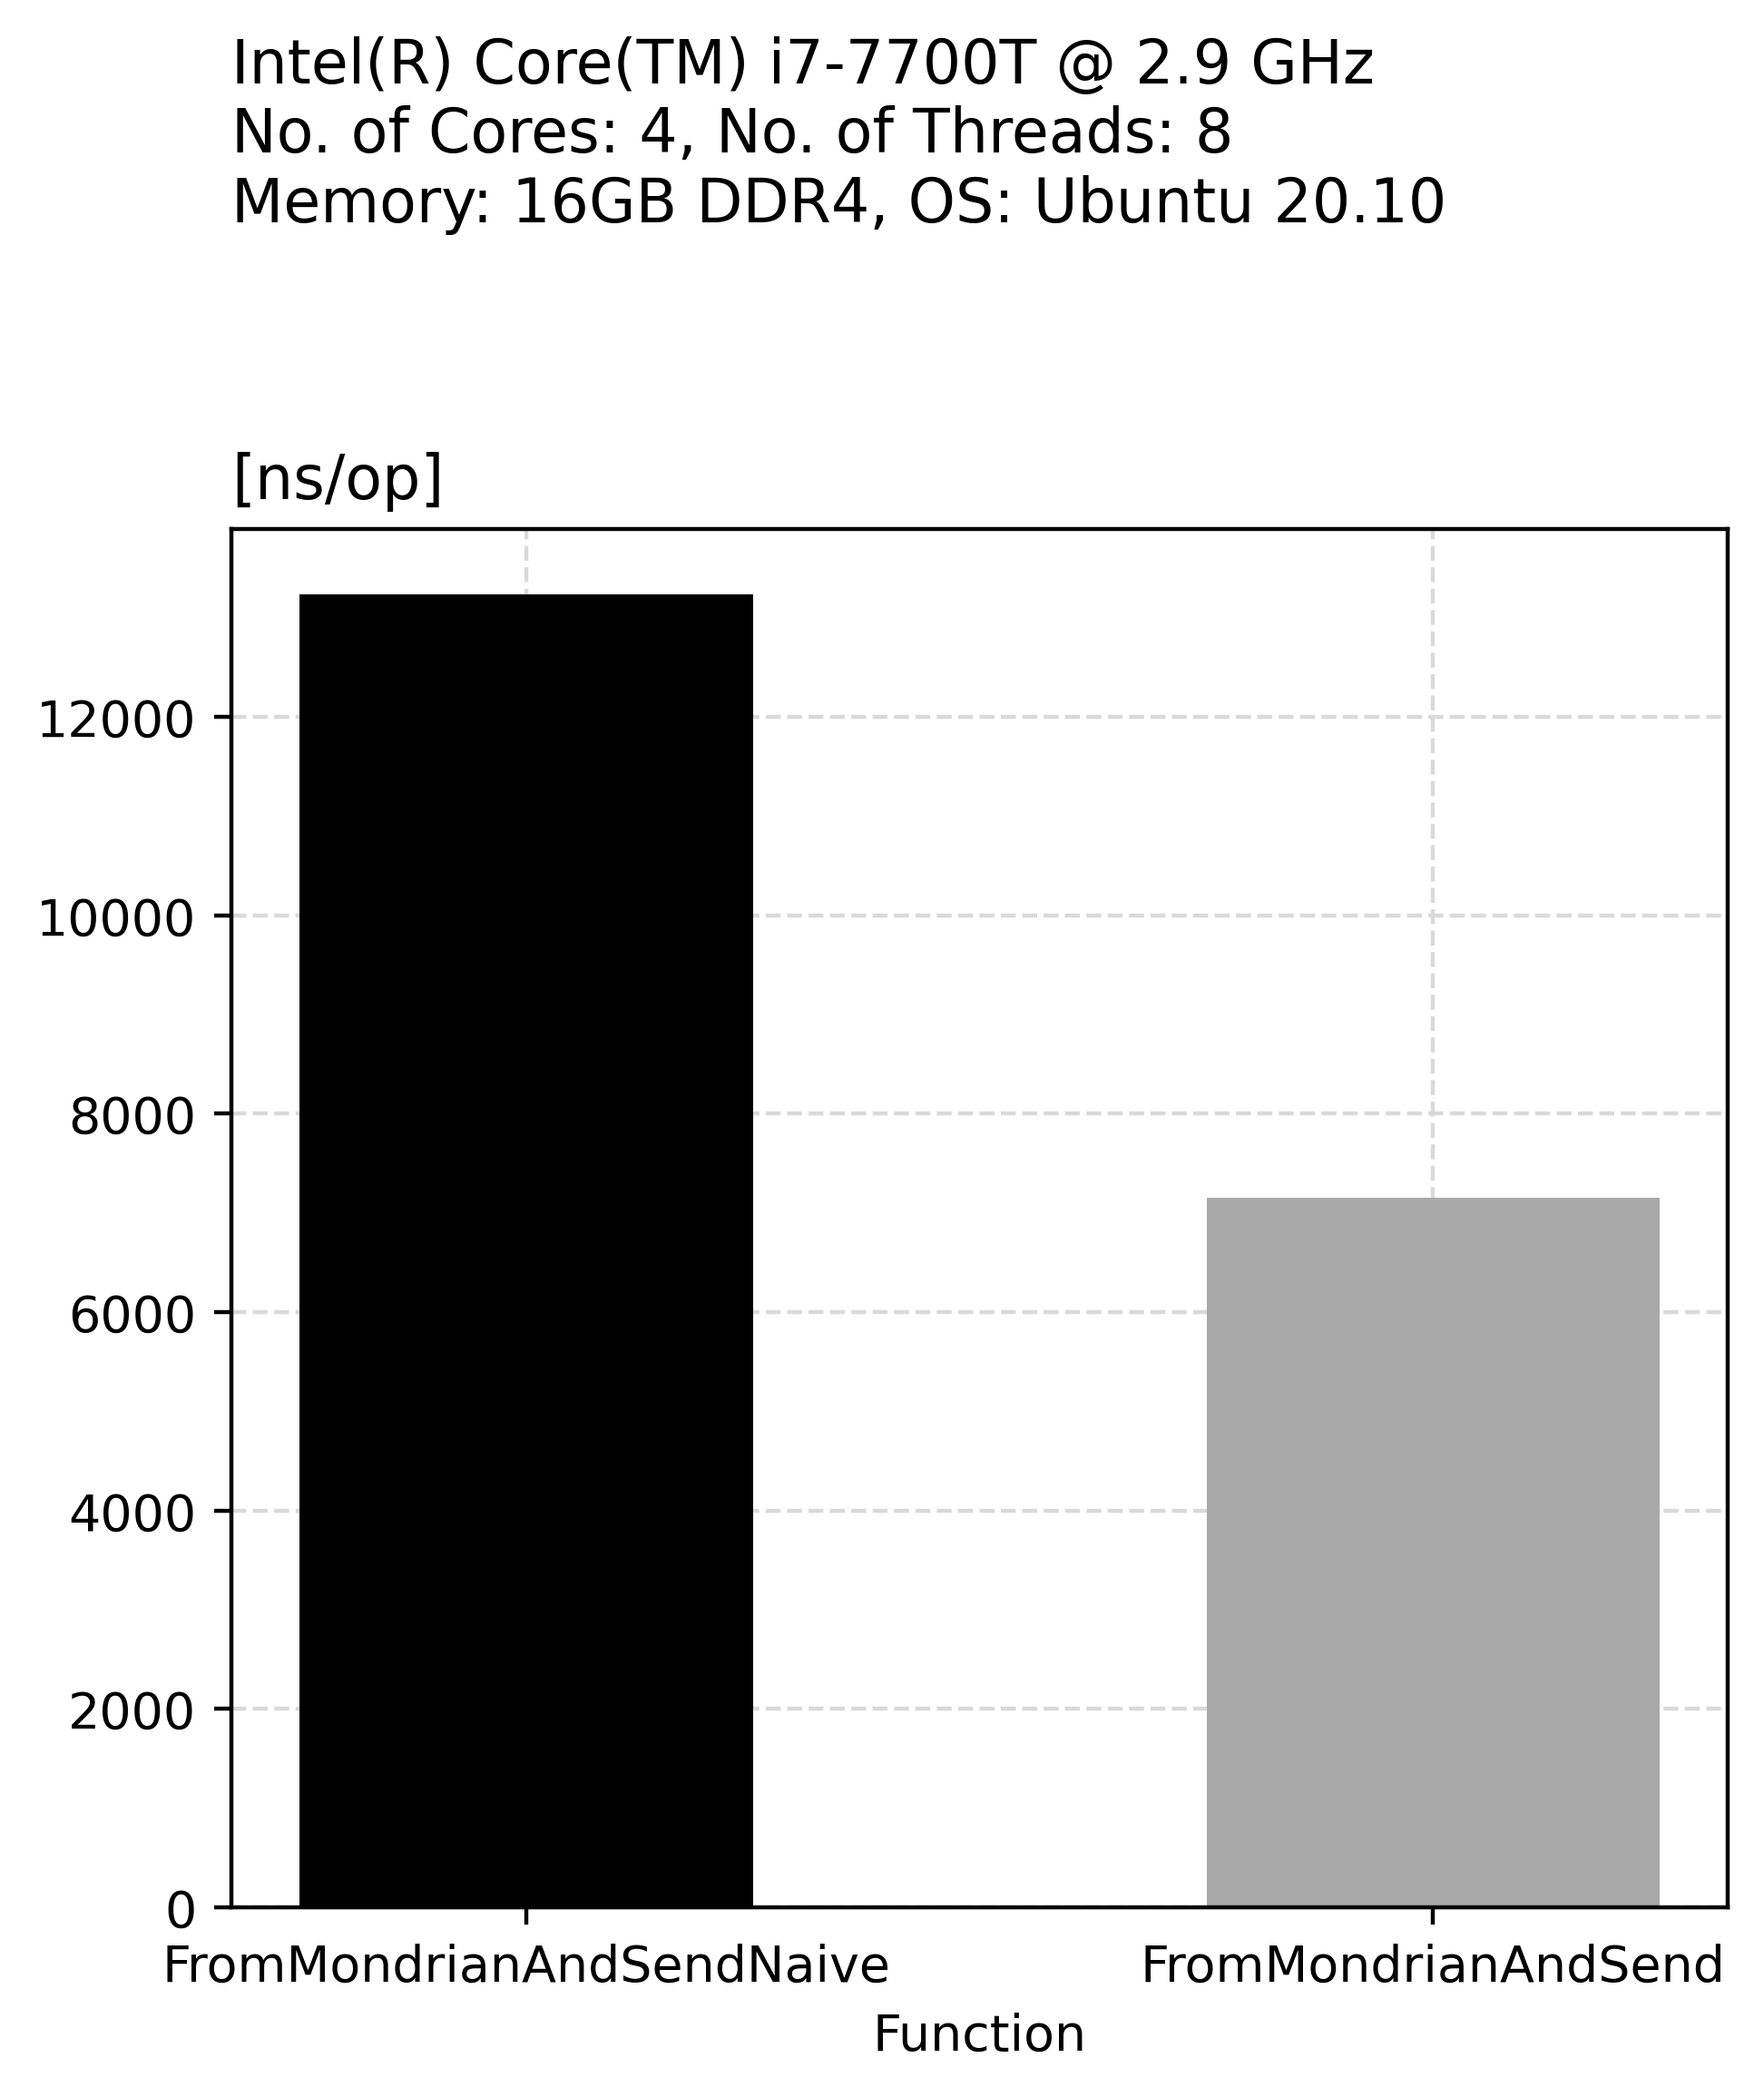
\includegraphics[width=\linewidth]{img/from_mondrian_and_send_opt_time.png}
      \caption{Latency Improvement}
      \label{fig:sub2: Latency Improvement}
    \end{subfigure}\hfill%
    \begin{subfigure}[t]{.22\textwidth}
      \centering
      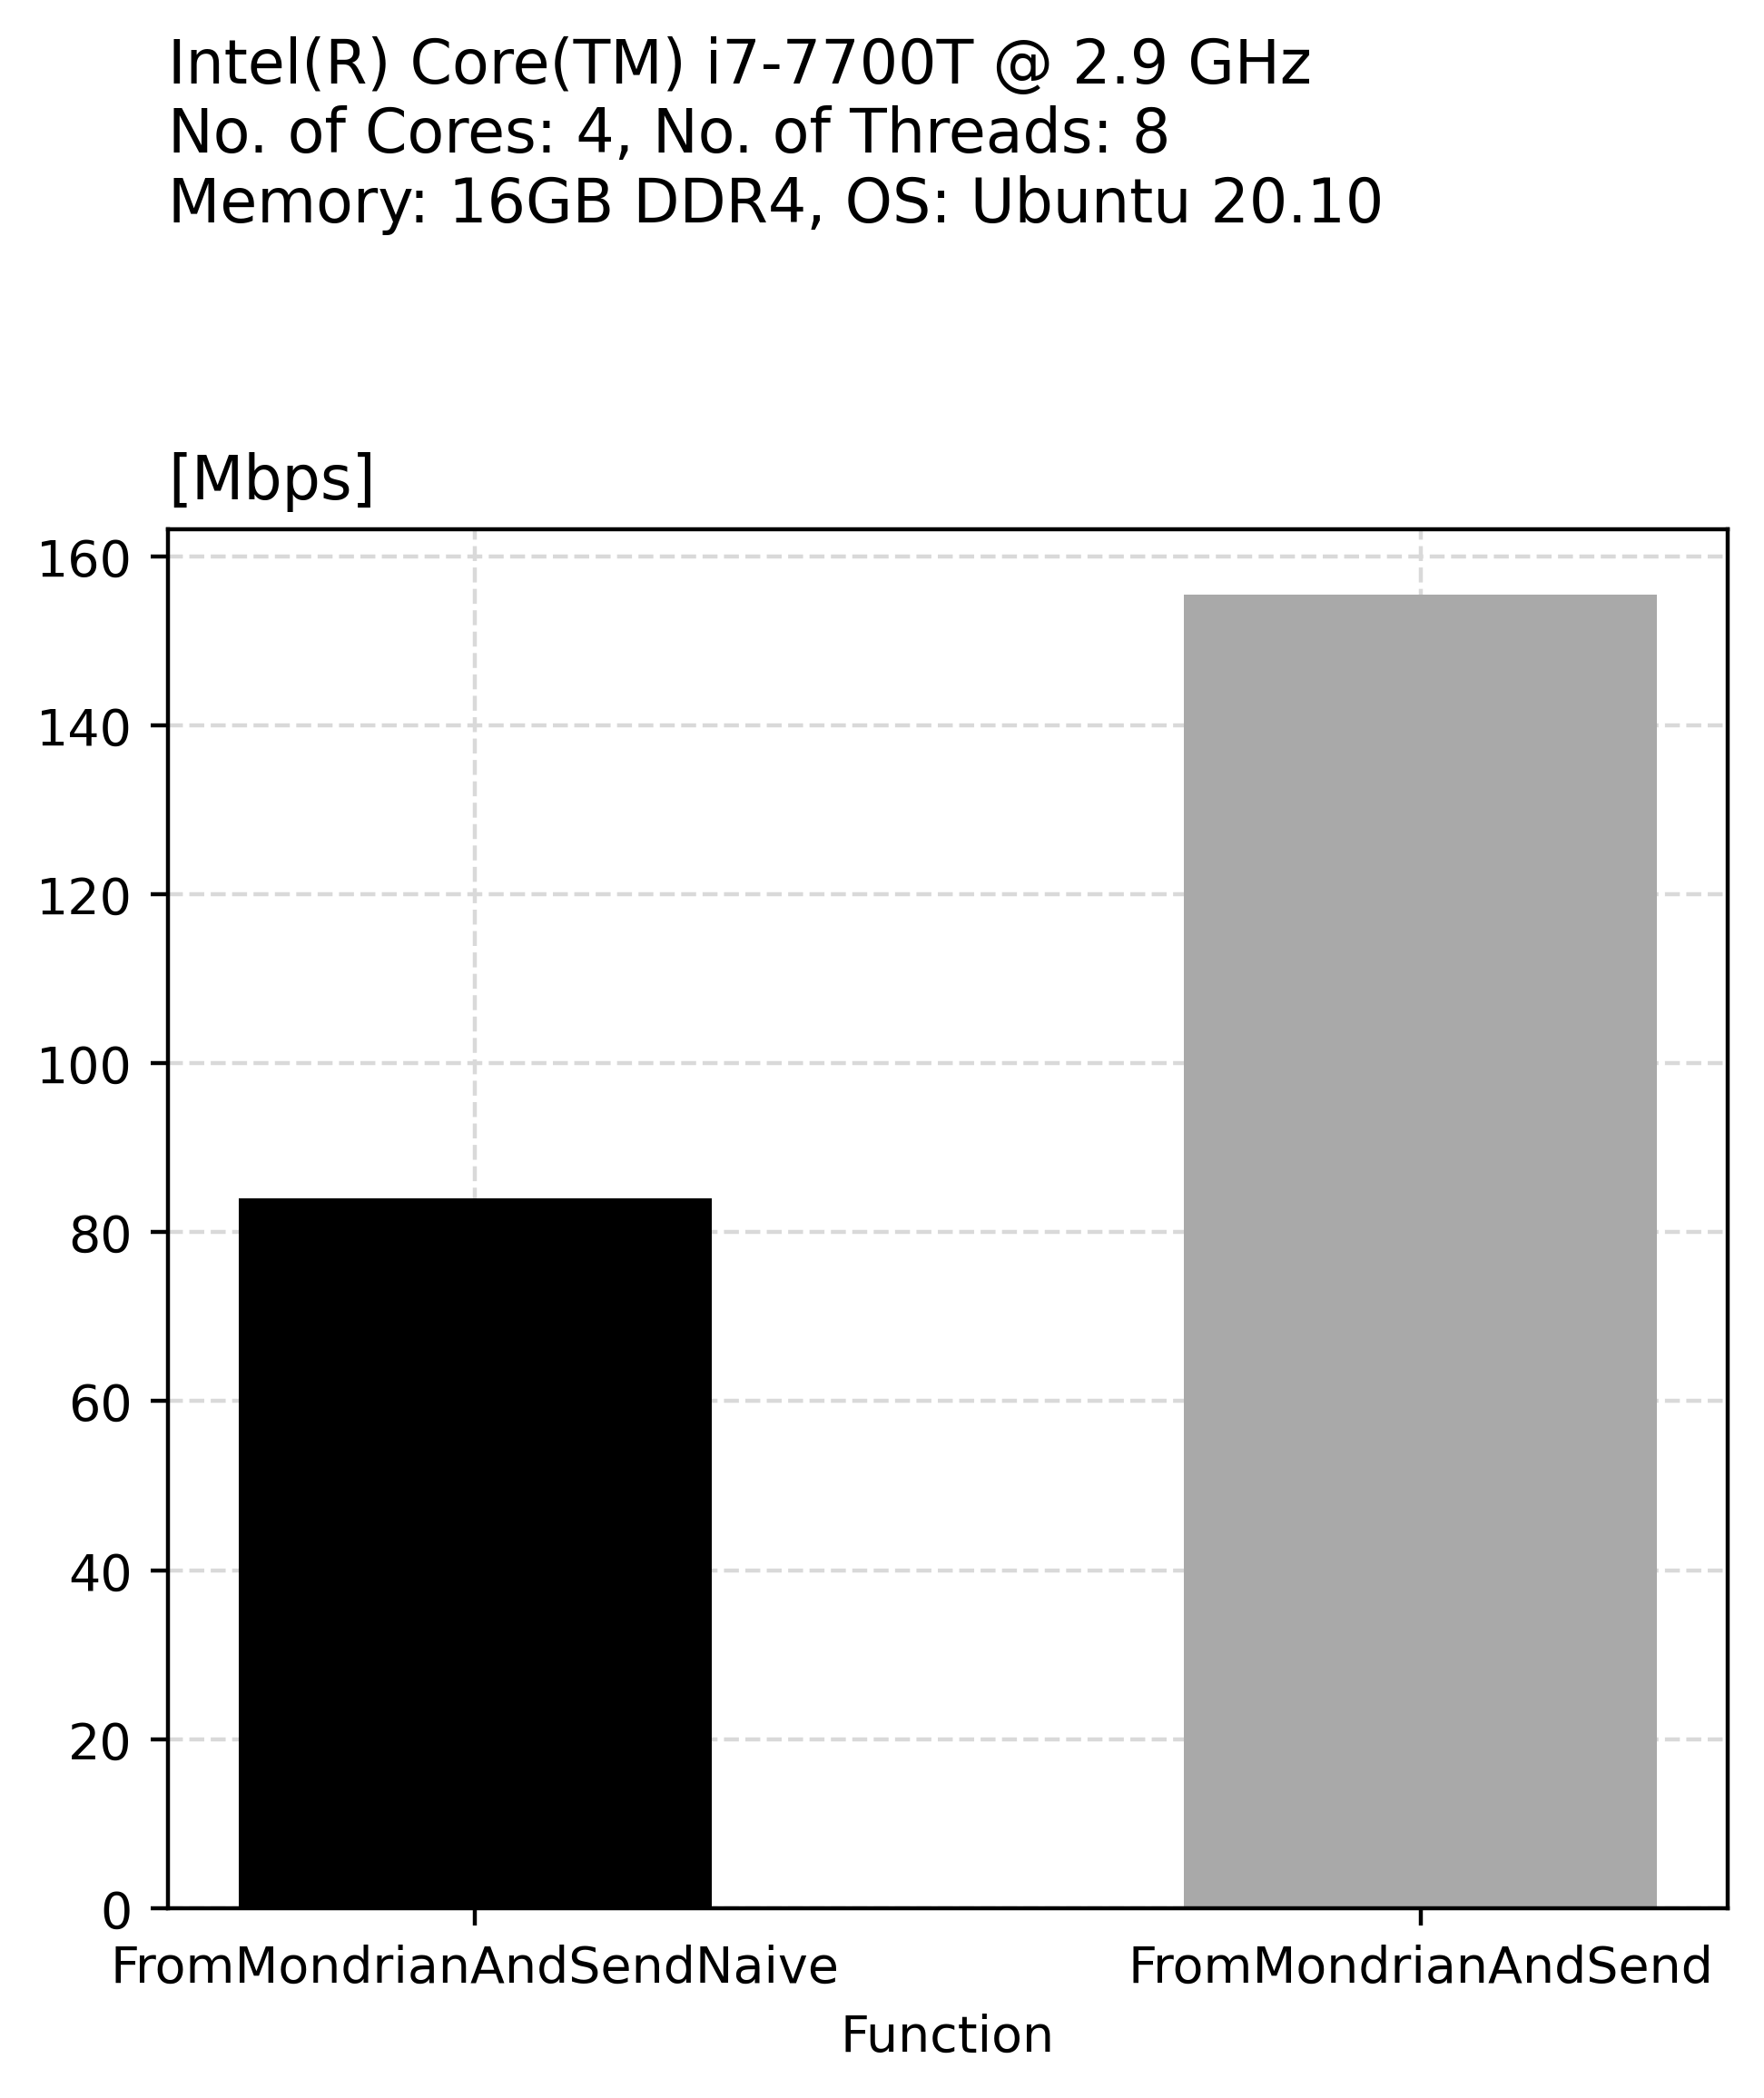
\includegraphics[width=\linewidth]{img/from_mondrian_and_send_opt_throughput.png}
      \caption{Throughput Improvement}
      \label{fig:sub2: Throughput Improvement}
    \end{subfigure}
    \caption{Microbenchmarking Results of the Performance Improvement in \texttt{FromMondrianAndSend} (thanks to \texttt{gopacket} related optimizations)}
    \label{fig:Performance Improvement in FromMondrianAndSend}
\end{figure}

% \clearpage
% \newpage
% \FloatBarrier
\subsection{Security Evaluation}\label{Security Evaluation}
\subsubsection{Threat Agents}\label{Threat Agents}
While there exist countless threat agents, few of them are of particular importance in the context of inter-domain network zoning in data centers.
\paragraph{Nation State Actors} As more and more important data from the private as well as from the public sector is migrated into the cloud, nation state actors have an increasing interest in spying on traffic between and within data centers. Espionage or sabotage operations are carried out in order to keep a competitive edge over rivaling powers.

\paragraph{Internet Service Providers} Many \acsp{ISP} (\aclp{ISP}) are partially or completely owned by nations. This means that they can't be trusted whenever the country in which they are based isn't trustworthy. Furthermore, \acsp{ISP} have monetary interests and might want to sniff on traffic to gain money through targeted advertising.

\paragraph{Competing Customers} Since data centers are multi tenancy environments, different customers of a data center might be competing companies. It therefore must be assumed that a host has an incentive to attack a different host of the same data center.  


\paragraph{Cyber Criminals} Just like any other computer network, data centers are targets of cyber criminals with monetary interests. Lots of valuable data is stored in data centers and the networks are usually enormous. It is therefore crucial, to provide a rigorous zoning mechanism to prevent lateral movement, originating from compromised hosts

%\todo{\\
%    - Many in general but some noteworthy\\
%    - Nation state adversary controling an ISP -- major reason why some sectors hesitate to move into a hybrid cloud model \\
%    - Competition which might try to compromise the availability of a competing service (can buy hosts in the same DC -- multy tenant environment)
%}
\subsubsection{Assets}
In the following subsections, we will discuss some of the most important assets we have to consider when doing our security evaluation. The intention is not to provide a full list of assets, but instead to focus on the most relevant ones. We group the assets into three different categories. Physical assets like physical machines, logical assets like software and information and finally intangible assets like confidentiality, integrity and availability (CIA triad).
\paragraph{Physical Assets}
Physical assets that we must take into consideration are the physical machines hosting the Gateway \acsp{TP}, the Endpoint \acsp{TP} together with the \acs{SDN} controller and the MONDRIAN Controller as well as the servers hosting the clients. The advantage of a data center and its heavily virtualized nature is that all these physical servers will most likely be the same or at least similar. Therefore, we just have to follow data center operator's best practices for providing safety and security for these physical assets. 
%\todo{Gateway TP Server, Endpoint TP Server/SDN controller, MONDRIAN Controller, Host machines}
\paragraph{Logical Assets}
Software wise, the most important asset we must consider is the entire software stack we utilize for the implementation of the MONDRIAN software portfolio. This includes the security of the programming languages, frameworks and libraries that we used, as well as the \acs{SDN} controller, the OpenFlow protocol and the \acs{SDN} switches. Since \acs{SDN} is heavily used in modern data centers, we should use the technologies that are already in place, since they have proven to be reliable and are well maintained, which improves the security of the overall system.

Regarding information assets, we must consider data at rest, as well as in transit. Data at rest is shielded from unauthorized access thanks to MONDRIAN's zone isolation properties. Data in transit consists of control plane traffic and data plane traffic. Control plane traffic is secured by using state of the art encryption protocols. In our case it is \acs{TLS}, but it could be any other protocol that might come up in the future. Inter-domain data plane traffic is encrypted and authenticated by using standard \acs{AES} encryption in \acs{GCM} mode. Additionally, we also have to consider the security of keys and certificates. We assume that the certificates are provided via a secure \acs{PKI}, which is already in place in modern data centers. Symmetric keys are dynamically created according to the \acs{DRKey} derivation scheme, which is also used in other protocols and is believed to be secure.
%\todo{Software of MONDRIAN software portfolio, SDN Controller + Openflow protocol+switches, information: Data at rest and in transit}
\paragraph{Intangible Assets}
The intangible assets we need to take into consideration are confidentiality and integrity of inter-domain traffic, isolation between different MONDRIAN zones as well as the availability of both intra- and inter-domain traffic. Confidentiality and integrity of inter-domain traffic is provided by using an \acs{AEAD}, which is based on \acs{AES} in \acs{GCM} mode. Isolation between MONDRIAN zones is provided if MONDRIAN is deployed correctly, meaning that the order of the \acs{SFC} is respected and all relevant switches are connected to an Endpoint \acs{TP}. The availability of services in a data center that is using MONDRIAN could be compromised in case of a \acs{DDoS} (\acl{DDoS}) attack. We will discuss that further in sections \ref{Security Improvements} and \ref{New Attack Vectors}.
%\todo{Confidentiality + authenticity of inter domain traffic, isolation of zones, availability of intra and inter domain traffic}

\subsubsection{Attacker Model}
As we discussed in section \ref{Threat Agents}, nation state actors as well as \acsp{ISP} are amongst the relevant threat agents. It therefore must be assumed that the entire inter-domain network, whether it is the public internet or an \acs{MPLS} (\acl{MPLS}) network doesn't make a huge difference, is not trustworthy and might be under the adversary's control. This means that we consider a standard Dolev-Yao attacker on the inter-domain network.

Furthermore, we saw in section \ref{Threat Agents} that the customers of a data center can't trust each other. This means that on the internal network we assume to have zones with compromised hosts, which completely control the virtual machine but can't compromise any networking components or the hypervisor.

Finally we assume to have perfect cryptography, meaning that encryptions can't be broken and signatures and \acsp{MAC} can't be forged.

%\todo{\\
%    - Dolev-Yao on the network \\
%    - Malitious customers (compromised hosts) \\
%    - Perfect Crypto \\
%}
\subsubsection{Security Improvements}\label{Security Improvements}
When comparing the new MONDRIAN design with the original one, there are two main security improvements that come with the new design. 

Firstly, the design of the Gateway \acs{TP} is much leaner than the one of the \acs{TP} from the original MONDRIAN design. This has the advantage that the attack surface is reduced, which is particularly important for the Gateway \acs{TP} due to its exposure to the public internet. If an attacker (either from the inside or outside of the data center) tries to compromise the availability of the data center by mounting a volumetric \acs{DDoS} attack on the system, it is an advantage to have a more performant Gateway \acs{TP}. Furthermore, not being in charge of performing zone transition authorization also means that no state needs to be kept. This improves the scalability of a Gateway \acs{TP} compared to the one of a traditional \acs{TP}, which in turn again makes the system more resilient to volumetric \acs{DDoS} attacks, since new instances of Gateway \acsp{TP} could be started up in a matter of seconds.

Secondly, the original MONDRIAN design does not provide egress filtering within the local domain. While unauthorized traffic is prevented from traversing the inter-domain connections, it could still cause congestion in the local network when it is routed to the \acs{TP}. In the new design, unauthorized traffic gets blocked at the first \acs{SDN} switch, which is connected to an Endpoint \acs{TP}, which is usually the virtual switch of the hypervisor. This prevents unauthorized traffic from using bandwidth in the data center's network and therefore reduces the risk of a volumetric DDoS attack of a host targeting the data center's network.

%\todo{\\
%    - Simpler Gateway TP reduces attack surface from the outside world\\
%    - Egress filtering right at the hypervisor prevents network congestion 
%    in the DC network fabric and prevents unauthorized traffic from using costly bandwidth 
%    (especially over expensive leased lines)
%}
\subsubsection{New Attack Vectors}\label{New Attack Vectors}
The new MONDRIAN design provides the same security properties regarding confidentiality, integrity and end-host anonymity of inter-domain traffic as the original MONDRIAN design. It also provides the same level of zone isolation, which means that new attack vectors can mainly be found when analyzing the new \acs{SDN} based design principles and their effect on the availability of the system. 

An attacker controlling a host in a data center could try to mount a \acs{DDoS} attack on the MONDRIAN deployment, by artificially crafting traffic that generates a maximum number of packet-in messages. Such a traffic pattern could for example be traffic, where each packet has a different source port. In that case, each packet would cause a flow table miss and trigger a packet-in message. A different candidate for a malicious traffic pattern would be replies to a connection, which hasn't been initialized but would be allowed, due to an established rule, if it had been initialized. Such packets can't be blocked on the \acs{SDN} switches since it's the Endpoint \acs{TP}'s responsibility to check in the connection state if such a connection has been initialized.

The first attack could be mitigated by simply deciding to not check certain properties. It is questionable, if a data center operator even needs to enforce policies based on the source port, since they are often chosen arbitrarily. If the operator decides not to check the source port then it should be possible to omit that check.

For the second attack vector, a mitigation technique would be to be more thoughtful in the policy making process. If the destination of a policy with \textit{established} as an action is trustworthy and won't mount such an attack, then such a policy will not cause any problems. However, for untrusted zones, established policies with these zones as destination zones should be avoided.

Note that both attacks can easily be detected, by logging and analyzing packet-in messages on the Endpoint \acs{TP} and could alert an administrator, which could then take the aforementioned countermeasures if desired.

%\todo{\\
%    - specially crafted traffic could cause many packet-in messages and DDoS the Endpoint TP\\
%    - Unwise policy decissions can increase the workload on the Endpoint TPs (wildcards 
%    should be avoided -- in some situations not checking some fields might make sense (srcPort))
%}